
\documentclass[11pt]{article}
\usepackage[left=4mm, right=4mm, top=3mm, bottom=7mm,paperwidth=140mm, paperheight=297mm]{geometry}

\usepackage[utf8x]{inputenc}
\usepackage{amssymb, amsfonts, amsmath, esint}
\usepackage{xcolor}
\usepackage[e]{esvect}
\usepackage{floatrow} % allows to insert pictures into proofs and theorems
\usepackage{cancel}
\usepackage{graphicx}
\usepackage{tabularx}
\usepackage{mwe} % for blindtext and example-image-a in example
\usepackage{wrapfig}
\usepackage{framed}
\usepackage{booktabs}
\usepackage[english,german,swissgerman]{babel} 
\usepackage{array}
\usepackage{enumitem}
\usepackage{float}
\usepackage{cancel}
\usepackage{multirow}
\usepackage{multicol}
%%From KomAZSF
\usepackage{amscd, amsmath, amssymb, blindtext, empheq, enumitem, multicol, parskip, esint}
\usepackage{mathtools}
\usepackage{graphicx}
\usepackage{tikz}
\usepackage{array} %for bigger tabular spacings
\usepackage{extarrows} % for arrows with text under and over them
\usepackage{mathrsfs} % for different math letters
\usepackage{xfrac} % for nice number fractions
\usepackage{trfsigns} % for laplace sign
\usepackage{pdfpages}





% Style Sheet
% use greek letters for phi and epsilon
\renewcommand{\phi}{\varphi}
\renewcommand{\epsilon}{\varepsilon}

% bolds math symbols
\newcommand{\bs}{\boldsymbol}
% Shortcut to write caligraphic math symbols
\newcommand{\mc}{\mathcal}
% norm
\newcommand{\norm}[1]{\left| \!\:\! \left| #1 \right| \!\:\! \right|}

% some shortcuts
\newcommand{\ds}{\displaystyle}
\newcommand{\arr}{\rightarrow}
\newcommand{\Arr}{\Rightarrow}
\newcommand{\LRA}{\Leftrightarrow}
\newcommand{\LLRA}{\Longleftrightarrow}
\newcommand{\nop}[1]{}
\newcommand{\rank}{\operatorname{rank}}
\newcommand{\cond}{\operatorname{cond}}
\newcommand{\grad}{\operatorname{grad}}
\newcommand{\argmin}{\mathop{\mathrm{argmin}}}
\newcommand{\argmax}{\mathop{\mathrm{argmax}}}
\newcommand{\mx}{\mathop{\mathrm{max}}}
\newcommand{\bigcupdot}{\bigcup \hspace{-0.35cm} \cdot}

\newcommand*\conj[1]{\overline{#1}}
\newcommand*\abs[1]{\vert #1 \vert}
\newcommand*\floor[1]{\lfloor #1 \rfloor}
\newcommand*\set[1]{\lbrace #1 \rbrace}
\newcommand{\eqdef}{\xlongequal{\text{def}}}
\newcommand{\lims}{\lim_{x \rightarrow x_0}}
\newcommand*\seq[1]{(#1)_{n = 0}^{\infty}}
\newcommand{\sinx}{sin(x)}
\newcommand{\siny}{sin(y)}
\newcommand{\cosx}{cos(x)}
\newcommand{\cosy}{cos(y)}
\newcommand{\tanx}{tan(x)}
\newcommand{\tany}{tan(y)}

% stuff for integrals
\newcommand{\intl}{\int\limits}
\newcommand{\rmd}{\mathrm{d}}
\newcommand{\rmD}{\mathrm{D}}

% number sets
\newcommand{\R}{\mathbb{R}}
\newcommand{\E}{\mathbb{E}}
\newcommand{\Z}{\mathbb{Z}}
\newcommand{\N}{\mathbb{N}}
\newcommand{\Q}{\mathbb{Q}}
\newcommand{\C}{\mathbb{C}}
\newcommand{\K}{\mathbb{K}}
\newcommand{\M}{\mathbb{M}}

% big-o notation
\newcommand{\bigO}{\mathcal{O}}

% 'with' in set notation
\newcommand{\with}{\;|\;}

% hyperref
\usepackage[colorlinks=false,pdfborder = {0 0 0 0}]{hyperref}


\colorlet{shadecolor}{orange!15}
\columnsep24pt
\columnseprule0.1pt

\setlength{\parindent}{0px}
\setlength{\parskip}{5px}
\setlength{\parsep}{0px}
\setcounter{secnumdepth}{4}

%% Redefine the \paragraph command:
\makeatletter
\renewcommand\paragraph{\@startsection{paragraph}{4}{0mm}%
	{-\baselineskip}%
	{0.5\baselineskip}%
	{\normalfont\bfseries}%
}%
\makeatother 

% algorithms
\usepackage{algorithmic}
\usepackage{algorithm}
\algsetup{linenodelimiter=}

% listings
\definecolor{darkgreen}{RGB}{0,127,14}
\definecolor{purple}{RGB}{75,0,130}
\usepackage{listings}


\usepackage{listings}
\usepackage{xcolor}
\lstset { %
    language=Pascal,
    backgroundcolor=\color{black!5}, % set backgroundcolor
    basicstyle=\footnotesize,% basic font setting
    escapeinside={!}{!},
    tabsize=2,
}

\def\doubleunderline#1{\underline{\underline{#1}}}

% theorem package
\usepackage{amsthm}
\usepackage{thmtools}
\newtheoremstyle{my-thm-style}% name
{6pt}% Space above
{5pt}% Space below
{}% Body font
{}% Indent amount
{\bfseries}% Theorem head font
{}% Punctuation after theorem head
{3pt}% Space after theorem head
{}% Theorem head spec (can be left empty, meaning `normal')

\definecolor{grey}{RGB}{40, 55, 71}
\definecolor{blue}{RGB}{93, 173, 226}
\definecolor{green}{RGB}{130, 224, 170}
\definecolor{red}{RGB}{229, 115, 115 }

\declaretheoremstyle[
headfont=\normalfont\bfseries,
notefont=\mdseries, notebraces={(}{)},
bodyfont=\normalfont,
postheadspace=8pt,
spaceabove=1pt,
mdframed={
  skipabove=2pt,
  skipbelow=2pt,
  hidealllines=false,
  backgroundcolor={blue!10},
  innerleftmargin=2pt,
  innerrightmargin=2pt}
]{def}

\declaretheoremstyle[
headfont=\normalfont\bfseries,
notefont=\mdseries, notebraces={(}{)},
bodyfont=\normalfont,
postheadspace=8pt,
spaceabove=1pt,
mdframed={
  skipabove=2pt,
  skipbelow=2pt,
  hidealllines=false,
  backgroundcolor={grey!10},
  innerleftmargin=2pt,
  innerrightmargin=2pt}
]{sat}

\declaretheoremstyle[
headfont=\normalfont\bfseries,
notefont=\mdseries, notebraces={(}{)},
bodyfont=\normalfont,
postheadspace=8pt,
spaceabove=1pt,
mdframed={
  skipabove=2pt,
  skipbelow=2pt,
  hidealllines=false,
  backgroundcolor={green!10},
  innerleftmargin=2pt,
  innerrightmargin=2pt}
]{lem}

\declaretheoremstyle[
headfont=\normalfont\bfseries,
notefont=\mdseries, notebraces={(}{)},
bodyfont=\normalfont,
postheadspace=8pt,
spaceabove=1pt,
mdframed={
  skipabove=2pt,
  skipbelow=2pt,
  hidealllines=false,
  backgroundcolor={green!0},
  innerleftmargin=2pt,
  innerrightmargin=2pt}
]{kor}

\declaretheorem[style=def, name=Def. , numberwithin=section]{definition}
\declaretheorem[style=sat, name=Satz, numberwithin=section]{satz}
\declaretheorem[style=lem, name=Lemma, numberwithin=section]{lemma}
\declaretheorem[style=kor, name=Korollar, numberwithin=section]{korollar}



%%%%%
\begin{document}
	
\setcounter{page}{1}
\setcounter{tocdepth}{2}


\title{Komplexe Analysis Zusammenfassung, ETH, D-INFK}
\author{Miles Strässle, Prof. A. Iozzi}
%\author{Simon Menzi, Prof. A. Iozzi}
\date{\today}
\maketitle
%\tableofcontents


% Use compiler for 3x1 Format on A4 Page, ask Author
% include the individual chapters
% \input{kap<n>.tex}
%\clearpage

%% Multiline-Comment
% \ifx true false
% ...
% \fi



\part{Zusammenfassung}
\input{src/src_koma/_TEMP_.tex}

\section{Komplexe Zahlen}

\begin{minipage}[c]{0.5\textwidth}
	\centering
	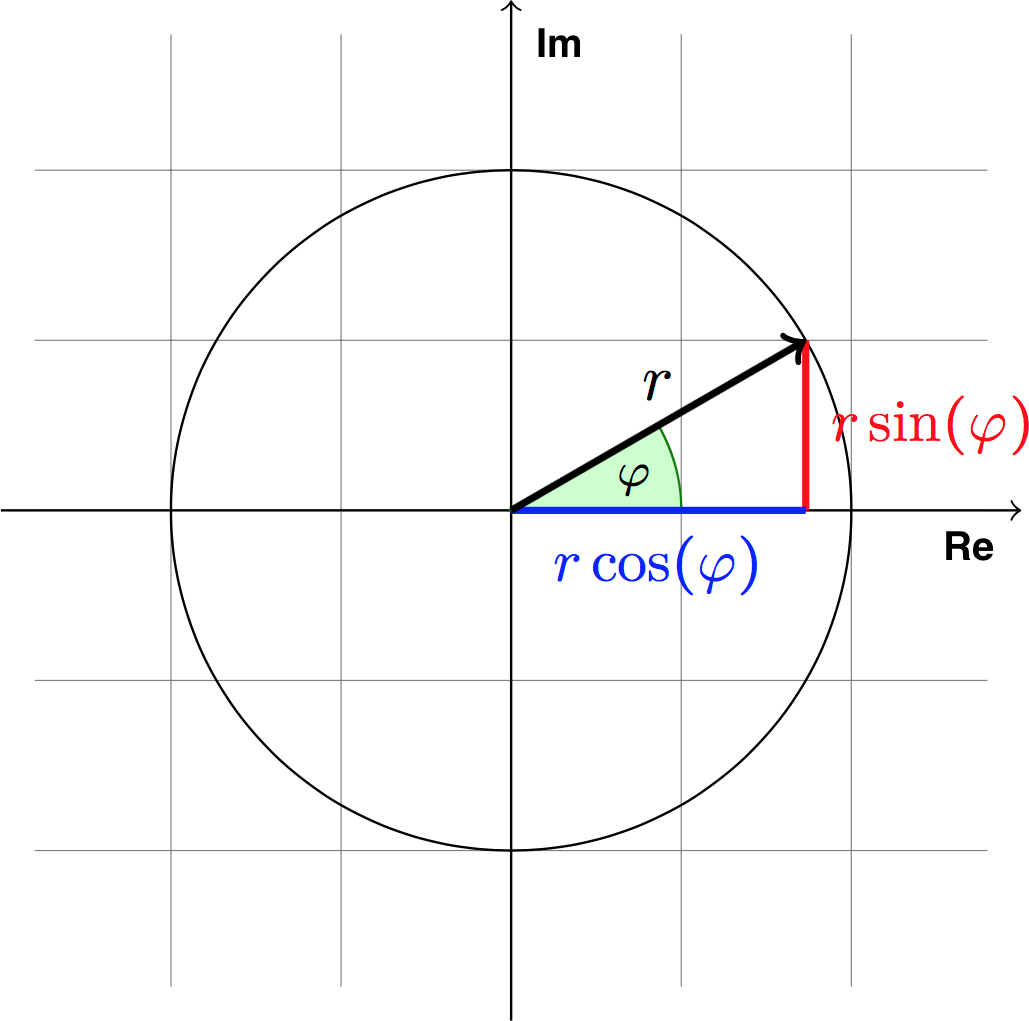
\includegraphics[width=\linewidth,keepaspectratio=true]{images/polarform}
\end{minipage}
%
\begin{minipage}[c]{0.5\textwidth}
	\begin{equation*}
	\begin{split}
	z & = x + iy = r(\cos(\varphi) + i\sin(\varphi)) = re^{i\varphi} \\
	r & = |z| = \sqrt{x^2 + y^2} \\
	\arg(z) & = \varphi  = \arctan(\frac{y}{x}) \quad \text{(je nach Quadrant)}  \\
	x & = r\cos(\varphi) \\
	y & = r\sin(\varphi) \\
	zw & = (re^{i\varphi})\cdot(se^{i\psi}) = rse^{i(\varphi + \psi)} \\
	\sqrt[q]{z} & = \sqrt[q]{s}e^{i\phi}\text{, wobei }\phi = \frac{\varphi}{q} \mod \frac{2\pi}{q} \\
	e^{i(\frac{\pi}{2} + 2\pi k)} & = i,\ e^{i\pi} = 1, \ e^{-i\pi} = -1
	\end{split}
	\end{equation*}
\end{minipage}

\begin{minipage}[c]{0.5\textwidth}
	\begin{equation*}
	\begin{split}
	(a,b) \cdot (c, d) & = (ac-bd, ad+bc) \\
	\overline{z} & = x - iy\\
	z^{-1} & = \frac{\overline{z}}{|z|^2} \\
	i & = \sqrt{-1}\\
	\end{split}
	\end{equation*}
\end{minipage}
%
\begin{minipage}[c]{0.5\textwidth}
	\begin{equation*}
	\begin{split}
	i^2 & = -1 \\
	|z|^2 & = z\overline{z} \\
	|zw|^2 & = (zw) \cdot \overline{(zw)} = |z|^2|w|^2
	\end{split}
	\end{equation*}
\end{minipage}
\figurename

\section{Komplexwertige Funktionen}
\textbf{Begriffe aus der Topologie}\\
\textbf{Umgebung}: (Beliebig kleine) Kreisscheibe um einen Punkt $z$.\\
\textbf{innerer Punkt}: Der Punkt $z$ befindet sich in einer Menge und ber"uhrt den Rand nicht (Umgebung um $z$ existiert in Menge).\\
\textbf{Randpunkt}: $z$ befindet sich auf dem Rand einer Menge.\\
\textbf{Ber"uhrungspunkt}: $z$ sitzt in oder auf dem Rand einer Menge.\\
\textbf{offene Teilmenge}: Teilmenge ohne Rand / nur innere Punkte\\
\textbf{abgeschlossene Teilmenge}: Teilmenge mit Rand / alle Ber"uhrungspunkte sind enthalten\\
\textbf{beschr"ankte Teilmenge}: F"ur jeden Punkt $z$ einer Teilmenge $S$ gilt: $\vert z \vert$ ist kleiner
als eine Konstante $M$.\\
\textbf{kompakte Teilmenge}: abgeschlossen und beschr"ankt.\\
\textbf{zusammenh"angende Teilmenge}: Jeder Punkt der Teilmenge kann mit jedem anderen Punkt der Menge nur "uber
andere Punkte der Menge verbunden werden (keine \"Inseln\").\\
\textbf{Gebiet}: zusammenh"angende offene Teilmenge.\\

\textbf{Komplexe Funktionen}\\
$f: \mathbb{R} \to \mathbb{C} $ oder $f: \mathbb{C} \to \mathbb{C} $\\
$f(z)$ ist das \textbf{Bild} von $z$ und $z$ ist das \textbf{Urbild} (nicht immer eindeutig) von $w = f(z)$.

\textbf{Hauptwert der $n$-ten Wurzel} (principal value, kurz: \textbf{pv}):\\
\fcolorbox{black}{formula}{
	\begin{tabular}{rl}
		pv $\sqrt[n]{w}$:
		& $\mathbb{C}^{-*} \to S = \lbrace z \in \mathbb{C}^* \vert -\frac{\pi}{n} < \text{Arg } z < \frac{\pi}{n} \rbrace$\\
		& $w \mapsto \sqrt[n]{\vert w \vert} e^{i\frac{\text{Arg } w}{n}}$
\end{tabular}}

\textbf{Komplexe Exponentialfunktion}\\
\eqbox{\text{exp }: \mathbb{C} \to \mathbb{C} \text{ , } z \mapsto w = \text{exp } z = \sum \limits_{k=0}^\infty \frac{1}{k!} z^k}\\
Es gelten folgende Umformungen:\\
\fcolorbox{black}{formula}{
	\begin{tabular}{l}
		$\text{exp}(z+z') = \text{exp }z \cdot \text{exp }z'$ mit $z,z' \in \mathbb{C}$\\
		$e^z = \text{exp }z$\\
		$e^{i\varphi} = \cos{\varphi} + i \sin{\varphi}$ f"ur reelle $\varphi$\\
		\emph{Aus letzterem folgt insbesondere}:\\
		$e^{2\pi i} = 1$ und\\
		$\text{exp}(z + 2\pi i) = \text{exp }z \cdot \text{exp}(2 \pi i) = \text{exp }z$
\end{tabular}}\\
$z ^\alpha = e^{\alpha log(z)}$\\					
\textbf{Logarithmus}\\
Da die Exponentialfunktion im komplexen periodisch ist, ist der komplexe Logarithmus als \textbf{Menge} definiert:\\
\eqbox{\log{w} = \lbrace z \in \mathbb{C} \text{ } \vert \text{ } e^z = w \rbrace \subseteq \mathbb{C}} \hspace{1cm} $\log(w) = \ln\vert w \vert + i \arg(w) $\\
Auch hier will man mit einem konkreten Wert rechnen k"onnen. Deshalb ist der \textbf{Hauptwert des Logarithmus} wie
folgt definiert:\\
\eqbox{\text{Log }: \mathbb{C}^{-* }\to \mathbb{C} \text{ , } w \mapsto \ln{\vert w \vert} + i \text{ Arg }w}\\
Hier ist Log nun injektiv und der \emph{eindeutig bestimmte Repr"asentant} von $\log w$ im Streifen
$S = \lbrace z=x+iy \vert - \pi < y < \pi \rbrace = \lbrace z \in \mathbb{C} \vert \text{ } \vert \text{Im }z \vert < \pi \rbrace $ 

\textbf{Potenz}\\
F"ur alle $a \in \mathbb{C}^{-*}$ (\underline{nur} f"ur diese!) ist der \textbf{Hauptwert der Potenz}:\\
\eqbox{\text{pv } a^z = \exp(z \text{Log } a)} und es gilt: \eqbox{\textbf{pv } a^{z+z'} = \textbf{pv }a^z \cdot \textbf{pv }a^{z'}}
%\newpage

\section{Die Cauchy-Riemannschen Differentialgleichungen}
Im folgenden untersuchen wir Real- und Imagin"arteil von \emph{analytischen} Funktionen ($f: \Omega \to \mathbb{C}$):\\
$ f = u(x,y) + i v(x,y) $ ($x+iy \in \Omega$)

Obige Funktion hat \emph{stetige partielle Ableitungen} nach $x$ und $y$ zwischen denen die \textbf{Cauchy-Riemannschen
	Differentialgleichungen} gelten:\\
\fcolorbox{black}{formula}{
	\begin{tabular}{c}
		$ u_x (x,y) = v_y (x,y) $\\
		$ v_x (x,y) = -u_y (x,y) $
\end{tabular}}
($x+iy \in \Omega$))\\

\textbf{Anwendung der CR-Differentialgleichungen}\\
Die CR-Differentialgleichungen in Polarkoordinaten sind:\\
\begin{tabular}{ccc}
	&\eqbox{u_r = \frac{1}{r} v_\varphi}	&	\eqbox{v_r = \frac{-1}{r} u_\varphi}\\
	\\
	&\eqbox{x = r \cos{\varphi}}		&	\eqbox{y = r \sin{\varphi}}\\
\end{tabular}

Zur Info: $holomorphie \Longrightarrow glattheit$\\
\fcolorbox{black}{formula}{
	\begin{tabular}{c}
		$u_x, u_y$ und $v_x, v_y$ existieren und erf"ullen\\
		die \emph{CR-Differentialgleichungen}\\
		$\Longleftrightarrow$\\
		$f(x+iy) = u(x,y) + iv(x,y)$ analytisch\\
		bzw. holomorph auf $\Omega$\\
		$\Longleftrightarrow$\\
		$ f' = f_x = u_x + iv_x $\\
		$ f' = -i f_y = v_y - i u_y $\\
		\(\GDW\)\\
		\(f\) komplex differenzierbar\\
		\(\GDW\)\\
		\(f\) \(\infty\)-mal komplex differenzierbar
\end{tabular}}					


\textbf{Beispiele}
\begin{itemize}
	\item $f(z) = \overline{z}$ ist \emph{nicht} differenzierbar, da die CR-Gleichungen nicht erf"ullt sind.
	\item \eqbox{f(z) = \vert z \vert^2 \text{ ist \textbf{keine analytische Funktion} im Ursprung}}.
	(Die Ableitung von $f$ existiert nur im Ursprung.) Eine Funktion heisst analytisch in $z_0$, falls sie in einer
	\emph{ganzen Umgebung} von $z_0$ analytisch ist.
	\item $\text{Log } z = \ln{\vert z \vert} + i \text{Arg }z$ ($z \in \mathbb{C}^{-*}$) ist analytisch auf $\mathbb{C}^{-*}$.
\end{itemize}

\section{Die Integralformel von Cauchy}
\subsection{Theorie "Ubung}
\textbf{Integral reeller Variablen ("'\(dx\)"' ist hier reell)}\\
\(g: \mathbb{R} \to \mathbb{C}\), dann:\\
\(\int\limits_a^b g(x) \text{ d}x = \text{"'Wie im reellen"'}
= \int\limits_a^b \text{Re}(g(x))\text{ d}x + i \int\limits_a^b \text{Im}(g(x))\text{ d}x\)

Regeln:\\
\(\left\vert \int\limits_a^b f(x) \text{ d}x \right\vert \leqslant \int\limits_a^b\vert f(x) \vert \text{ d}x\)
und \(\overline{\int\limits_a^bf(x)\text{ d}x} 	= \int\limits_a^b \overline{f(x)} \text{ d}x\)

\textbf{Eine Kurve / ein Weg}\\
\(\gamma: [a,b] \to \mathbb{C}\) stetig und st"uckweise glatt

Spur von \(\gamma\): \(\text{sp}(\gamma)=\{\text{Menge aller Bildpunkte von }\gamma\}\)

\textbf{L"ange der Kurve}: \eqbox{= \int\limits_a^b \vert \dot \gamma(t) \vert \text{ d}t}

\textbf{Komplexes Linienintegral der Funktion \(f\) "uber der Kurve \(\gamma\)}\\
\(f: \mathbb{C} \to \mathbb{C}\), Parametrisierung \(\gamma: [a,b] \to \mathbb{C}\); dann gilt:\\
\eqbox{\int\limits_\gamma f(z) \text{ d}z = \int\limits_a^b f(\gamma(t))\cdot \dot \gamma(t) \text{ d}t}
wobei \(\text{d}t\) wieder reell ist.

Es gilt: \eqbox{\int\limits_{-\gamma} f(z) \text{ d}z = -\int\limits_\gamma f(z) \text{ d}z}

\textbf{Parametrisierungen}\\
(k"onnen auch AUFGETEILT werden: \(\gamma = \gamma_1 + \gamma_2\))\\
\emph{Gerader / direkter Weg} von \(a\) nach \(b\):\\
\eqbox{\gamma(t) = a(1-t)+bt=a+t(b-a) \quad 0\leqslant t<1 \quad \dot \gamma(t) = b-a}

Kreis \textbf{gegen} den Uhrzeigersinn mit Radius \(r\) um Mittelpunkt \(a\):\\
\eqbox{\gamma(t) = a+re^{it} \quad 0 \leqslant t < 2\pi \quad \dot \gamma(t) = ire^{it}}

Einheitskreis \textbf{im} Uhrzeigersinn um den Ursprung \((a=0)\):\\
\eqbox{\gamma(t) = 1\cdot e^{-it} \quad 0 \leqslant t < 2\pi \quad \dot \gamma(t) = -ie^{-it}}

Funktion \(y=f(x)\):\\
\eqbox{\gamma(t)=f(t)}

\textbf{Satz von Cauchy}\\
Sei \(\Omega\) ein \emph{einfach zusammenh"angendes} Gebiet (= offen, keine L"ocher) und \(f: \Omega \to \mathbb{C}\)
\emph{analytisch}. Dann gilt f"ur jede geschlossene Kurve ("'Zyklus"')" \(\gamma\) mit \(a=b\):
\eqbox{\oint\limits_\gamma f(z) \text{ d}z = 0}

und deshalb folgt f"ur alle Kurven \(\gamma_1\) und \(\gamma_2\) mit demselben Anfangspunkt \(a\) und Endpunkt \(b\):\\
\eqbox{\int\limits_{\gamma_1} f(z) \text{ d}z = \int\limits_{\gamma_2} f(z) \text{ d}z}\\
\(\implies\) Der Wert des Integrals ist \textbf{WEGUNABH"ANGIG}!


\textbf{Integralsatz von Cauchy}\\
\(f: \Omega \to \mathbb{C}\) analytisch, \(\Omega\) einfach zusammenh"angend, \(\gamma\) ein beliebiger Zyklus welcher
den Punkt \(a\in\Omega\backslash \text{sp}(\gamma)\) \(n(\gamma,a)\)-mal \emph{gegen den Uhrzeigersinn} uml"auft:\\
\eqbox{\int\limits_{\gamma} \dfrac{f(z)}{z-a} \text{ d}z = 2 \pi i \cdot n(\gamma,a) \cdot f(a)}

\textbf{Integralsatz von Cauchy f"ur h"ohere Ableitungen}\\
Sei \(f\) analytisch auf ganz \(\Omega\) und \(K\) eine Kreisscheibe innerhalb von \(\Omega\) mit Rand \(\partial K\) (hier wird
im Gegenuhrzeigersinn dar"uber integriert!).
Dann gilt f"ur alle \(n\geqslant 0\):\\
\eqbox{f^{(n)}(a)\cdot n(\gamma,a) = \dfrac{n!}{2 \pi i} \int\limits_{\partial K} \dfrac{f(z)}{(z-a)^{n+1}} \text{ d}z}

Analog:\\
\eqbox{\dfrac{2 \pi i}{n!} f^{(n)}(a)\cdot n(\gamma,a) = \int\limits_{\partial K} \dfrac{f(z)}{(z-a)^{n+1}} \text{ d}z}
%\newpage
\subsection{Mittelwertsatz}
Seien $ U ⊂ \mathbb{C}$ eine offene Menge und $f : U \rightarrow \mathbb{C}$ eine holomorphe Funktion. Seien $z_0 \in U$ und $r > 0$ so dass $B(z_0, r) \subseteq U$ . Dann gilt:\\
\eqbox{f(z_0) = \int\limits_0^1 f(z_0 + r exp(2 \pi it)) dt}\\
d.h. $f(z_0)$ ist der Mittelwert von f auf dem Kreis mit Zentrum $z_0$ und Radius r

\subsection{Maximum Modulus Prinzip}
Sei f holomorph und nicht konstant auf einer wegzusammenha"ngenden Menge U. Dann besitzt $|f (z)|$ kein Maximum
auf U . Anders gesagt, gibt es keinen Punkt $z_0 \in U$ mit $|f (z)| ≤ |f (z_0 )|.$


\section{Reihen}
\subsection{Gew"ohnliche Reihen und Potenzreihen}
\begin{tabular}{ll}
	\textbf{Gew"ohnliche Reihe}			&	\textbf{Potenzreihe} (mit Entwicklungspunkt \(z_0\))\\
	\(\sum\limits_{k=0}^\infty a_k\)			&	\(\sum\limits_{k=0}^\infty b_k (z-z_0)^k\)
\end{tabular}

\textbf{"Uberf"uhren der beiden verschiedenen Reihen}\\
Wir k"onnen immer \(z_0=0\) annehmen oder \(w=z-z_0\) substituieren und erhalten dann:\\
\eqbox{\sum\limits_{k=0}^\infty a_k = \sum\limits_{k=0}^\infty b_k z^k} mit \(a_k = b_k z^k\)

\subsection{Konvergenzradius (f"ur alle Reihen)}
Der Index (\(k=\dots\)) ist f"ur den Konvergenzradius \textbf{nicht relevant}! (Kann z.B. auch \(k=2\) sein.)

\emph{Quotientenkriterium}:\\
\(\lim\limits_{n\to \infty} \dfrac{a_{n+1}}{a_n} = q \in \mathbb{C}\)\\
\(\implies \begin{cases}
\sum\limits_{n=0}^\infty a_n \text{konvergiert absolut, falls }\vert q \vert < 1\\
\sum\limits_{n=0}^\infty a_n \text{divergiert, falls }\vert q \vert > 1\\
\end{cases}\)

\emph{Wurzelkriterium}:\\
\(q=\lim\limits_{n\to\infty} \sqrt[n]{\vert a_n \vert}\)\\
und die Reihe konvergiert f"ur \(q<1\) und divergiert f"ur \(q>1\).

\subsection{Potenzreihen}
\textbf{Form} \eqbox{ f(z) = \sum_{k=0}^{\infty} a_k (z-z_0)^k }

\textbf{Ableitung}\\
\eqbox{f^{(n)}(z) = \sum_{k=n}^{\infty} k(k-1)\cdots (k-n+1)\cdot a_k (z-z_0)^{k-n}}

\subsection{Konvergenzradius (Potenzreihen)}
Potenzreihen konvergieren auf Kreisscheiben mit Konvergenzradius $\rho$:

\begin{tabular}{ll}
	\emph{Quotientenkriterium}							&	\emph{Wurzelkriterium}\\
	\eqbox{\rho = \lim_{k \rightarrow \infty} \frac{|a_k|}{|a_{k+1}|}}	&
	\eqbox{\rho = \frac{1}{\limsup\limits_{k \rightarrow \infty} \sqrt[k]{|a_k|}}}
\end{tabular}

Am Rand der Konvergenzkreisscheibe verhalten sich die Reihen unterschiedlich.



\subsection{isolierte Singularit"at (\(z_0\))}
\begin{enumerate}
	\item	\(z_0\) ist hebbar: \( \lim\limits_{z \to z_0} f(z) = \lambda \neq \pm \infty \)\\
	\(\to\) Hauptteil der Laurentreihe \emph{um} \(z_0\) ist null.\\
	(f analytisch fortsetzbar)\\
	falls $f(z)$ beschr"ankt in $\Omega \Rightarrow z$ ist eine hebb. Sing.
	\item	\(z_0\) ist Polstelle \(k\)-ter Ordnung:\\
	\( \lim\limits_{z \to z_0} (z-z_0)^k f(z) = \lambda \neq \pm \infty \text{ und } \neq 0
	\Longleftrightarrow k \geq \) Ordnung des Pols.\\
	\( \to \) Hauptteil der zugeh"origen Laurentreihe ist endlich lang\\
	\(k\) ist zu hoch gew"ahlt, falls der Grenzwert \(= 0\) ist und zu niedrig, falls der Grenzwert unendlich ist
	oder nicht existiert. Die tiefste Ordnung des Hauptteils entspricht \(k\).\\
	\textbf{Trick zur Bestimmung der Ordnung}: Die Ordnung ist gleich dem ersten \(k\) f"ur das gilt:
	\(f^{(k)}(z_0) \neq 0\).\\
	Falls $\lim\limits_{z \rightarrow z_0} |f(z)| = \infty \Rightarrow z_0$ ist eine Polstelle
	\item	\(z_0\) ist eine wesentliche Singularit"at:\\
	\( \lim\limits_{z \to z_0} (z-z_0)^k f(z)\) existiert f"ur kein \(k\). Funktion verh"alt sich chaotisch im Punkt \(z_0\).
	Der Hauptteil der Laurentreihe um \(z_0\) hat unendlich viele Elemente. Bsp.: \(\sum_{k=-\infty}^{-1} a_k (z-z_0)^k\)
\end{enumerate}

\subsection{nicht isolierte Singularit"at}
Hat keinen Typ. Bsp: \(z_0 = 0\) bei \(\dfrac{1}{\sin(\frac{1}{z})}\)


\section{Der Residuensatz}
\subsection{Residuensatz}
Sei $U \subseteq \mathbb{C} $ eine offene wegzusammenh"angende Teilmenge und sei $\gamma : [0, 1] \rightarrow U$ eine positiv orientierte einfache geschlossene Kurve. \\
Seien $z_1, ..., z_n$ im Innere von $\gamma$ enthalten und sei $f : U$ \textbackslash $ \{z_1 , ..., z_n \} \rightarrow \mathbb{C}$ holomorph. Dann gilt:
	
	

\(\displaystyle \oint\limits_{\partial \Omega} f(z) dz =
2\pi i \sum\limits_{z_i \in \Omega} \text{Res}\big(f \big\vert z_i\big) \cdot n(\gamma(t), z_i)\)\\
( \( n\left(\gamma (t), z_i\right) \text{ normalerweise} = \pm 1 \) )

\subsection{Residuenberechnung}
\begin{enumerate}
	\item	\eqbox{ \text{Res}\big(f \big\vert z_0\big) = \lim\limits_{z \to z_0}(z-z_0)f(z)}\\
	falls \(z_0\) ein \textbf{Pol erster Ordnung} ist.
	\item	\eqbox{ \text{Res}\big(f \big\vert z_0\big) = \lim\limits_{z \to z_0} \dfrac{1}{(m-1)!}\left(\dfrac{d}{dz}\right)^{m-1}
		\Big[(z-z_0)^m f(z)\Big]}\\
	falls \(z_0\) \textbf{Pol \(m\)-ter Ordnung}\\
	\item	\eqbox{ \text{Res}\big(f \big\vert z_0\big) = \dfrac{p(z_0)}{q'(z_0)}} \qquad falls \(f(z) = \dfrac{p(z)}{q(z)}\)\\
	und \(q(z)\) in \(z_0\) eine \textbf{einfache Nullstelle} hat.\\
	(\( p(z) \) und \( q(z) \) analytisch, aber nicht unbedingt Polynome!)
	\item	\( \text{Res}\big(f \big\vert z_0\big) = \) Koeffizienten von \(z^{-1}\) der innersten Laurentreihe
	um den Punkt \(z_0\). (=\(a_{-1}\))
	\item	\( \text{Res}\big(f \big\vert z_0\big) = \dfrac{1}{2\pi i} \oint\limits_{\partial B} f(z) dz \) \qquad
	mit \(\partial B = \partial B(z_0,r)\)
	\item	\( \text{Res}\big(f \big\vert z_0\big) = 0\)\\
	falls \(z_0 = 0\) und  \(f(z)\) gerade (Laurentreihe hat nur gerade Koeff.)
\end{enumerate}

\subsection{Integralabsch"atzungen}
\( \lim\limits_{R \to \infty} \left( \left\vert \int\limits_{S_R} f(z) dz \right\vert \right) \leqslant
\lim\limits_{R \to \infty} \pi \cdot R \cdot \max \left( \left\vert f(z) \right\vert \right) \)\\
wobei \(S_R =\) Halbkreis, \(R \to \infty\)

\( \displaystyle \lim_{\epsilon \to 0} \int_{\vert z-z_0 \vert = \epsilon, \text{Im}(z) > 0} f(z) dz
= \pi \cdot i \cdot \text{Res}\big(f \big\vert z_0\big) \)\\
(Halbkreis um Singularit"at)


\subsection{G"angster-Lemma}

Sei $\gamma_R (t) := Re^{ıt}$ f"ur $t \in [0, \pi].$ Seien p und q Polynome mit der
folgenden Eigenschaften:
\begin{enumerate}
	\item $deg(p) ≤ deg(q) − 2$;
	\item $q(x)$ besitzt keine Nullstellen auf der x-Achse.
\end{enumerate}
Sei $f(z) := \frac{p(z)}{q(z)} \cdot h(z)$, wobei $\vert h(z) \vert$ auf der Menge $\{  z \in \mathbb{C} : Im(z) \geq 0\}$ beschränkt ist. Dann gilt: $\lim_{R \rightarrow \infty} \int_{\gamma_R} f(z) dz = 0$




\subsection{Einige Anwendungen des Residuensatzes}
\begin{enumerate}
	\item \(\displaystyle \int\limits_0^{2\pi} f(\cos(\varphi),\sin(\varphi)) d\varphi
	= \dfrac{1}{i} \int\limits_{\vert z \vert = 1} \dfrac{1}{z} f \left(\dfrac{z+z^{-1}}{2}, \dfrac{z-z^{-1}}{2i}\right) dz \)\\
	\hspace*{1cm} \(\displaystyle = 2\pi \sum\limits_{z_i \in \partial B(0,1)}
	\text{Res}\big( \dfrac{1}{z} f\left(\dfrac{z+z^{-1}}{2}, \dfrac{z-z^{-1}}{2i}\right) \Big\vert z_i) \)
	
	\item	\( \displaystyle \int\limits_{-\infty}^\infty f(x) dx = \begin{cases}
	\displaystyle 2\pi i \sum\limits_{z_i \in H^+} \text{Res}\big(f \big\vert z_i\big)
	+ \pi i \sum\limits_{z_i \in \mathbb{R}} \text{Res}\big(f \big\vert z_i\big)	\\
	\displaystyle -2\pi i \sum\limits_{z_i \in H^-} \text{Res}\big(f \big\vert z_i\big)
	- \pi i \sum\limits_{z_i \in \mathbb{R}} \text{Res}\big(f \big\vert z_i\big)
	\end{cases}\)
	
	falls \( f(z) = \dfrac{p(z)}{q(z)}\) und \( \deg(p) \leqslant \deg(q) - 2 \)
	
	\item	\( \displaystyle \int\limits_{-\infty}^\infty f(x) e^{i\alpha x}dx = \begin{cases}
	\displaystyle 2\pi i \sum\limits_{z_i \in H^+} \text{Res}\big(f(z)e^{i\alpha z} \big\vert z_i\big)	&	\alpha \geqslant 0\\
	\displaystyle -2\pi i \sum_{z_i \in H^-} \text{Res}\big(f(z)e^{i\alpha z} \big\vert z_i\big)		&	\alpha \leqslant 0\\
	\end{cases} \)
	
	falls \( f(z) = \dfrac{p(z)}{q(z)} \) und \( q(z) \neq 0\)  \(\forall z \in \mathbb{R}\) und \( \deg(p) \leqslant \deg(q) - 2 \)
	
	\item	\( \displaystyle \int\limits_{-\infty}^\infty f(x) \cos(\alpha x)dx = \begin{cases}
	\displaystyle -2\pi\cdot \text{Im}\left(\sum_{z_i \in H^+} \text{Res}\big(f(z)e^{i\alpha z} \big\vert z_i\big) \right)
	&	\alpha \geqslant 0\\
	\displaystyle 2\pi\cdot \text{Im}\left(\sum_{z_i \in H^-} \text{Res}\big(f(z)e^{i\alpha z} \big\vert z_i\big) \right)
	&	\alpha \leqslant 0\\
	\end{cases} \)
	
	\(\to\) \emph{gleiche Bedingungen wie bei 3.}
	
	\item	\( \displaystyle \int\limits_{-\infty}^\infty f(x) \sin(\alpha x)dx = \begin{cases}
	\displaystyle 2\pi\cdot \text{Re}\left(\sum_{z_i \in H^+} \text{Res}\big(f(z)e^{i\alpha z} \big\vert z_i\big) \right)
	&	\alpha \geqslant 0\\
	\displaystyle -2\pi\cdot \text{Re}\left(\sum_{z_i \in H^-} \text{Res}\big(f(z)e^{i\alpha z} \big\vert z_i\big) \right)
	&	\alpha \leqslant 0\\
	\end{cases} \)
	
	\(\to\) \emph{gleiche Bedingungen wie bei 3.}
\end{enumerate}

Dabei ist mit $H^+$ die obere Halbebene, und mit $H^-$ die untere Halbebene gemeint. Also folgt:\\
\(z \in H^+\): Singularit"aten liegen auf der \textbf{oberen Halbebene}\\
\(z \in H^-\): Singularit"aten liegen auf der \textbf{unteren Halbebene}\\
\(z \in \mathbb{R}\): Singularit"aten liegen auf der \textbf{reellen Achse}\\






\section{Taylorreihe}
\eqbox{f(z) = \sum_{k=0}^\infty \frac{f^{(k)}(z_0)}{k!}(z-z_0)^k }\(\qquad \forall z \in B(z_0, \rho)\)

\subsection{Wichtige Potenzreihen}
\emph{geometrische Reihe}:\\
$\displaystyle \dfrac{1}{1-\left(\dfrac{z}{c}\right)^d} = \sum_{k=0}^\infty \left(\dfrac{z}{c}\right)^{d \cdot k}
\Longleftrightarrow \left\vert\dfrac{z}{c}\right\vert<1$ \qquad mit \(\rho = 1\)

$\displaystyle \dfrac{1}{c\left(1-\dfrac{z}{c}\right)^2} = \sum_{k=1}^\infty \dfrac{k}{c}\left(\dfrac{z}{c}\right)^{k-1}
\Longleftrightarrow \left\vert\dfrac{z}{c}\right\vert<1$ \qquad mit \(\rho = c\)

\emph{Wichtige Umformung f"ur geom. Reihe}:\\
\(\dfrac{1}{2-z} = \dfrac{1}{2-z+1-1}=\dfrac{1}{1-(z-1)} = \sum\limits_{k=0}^\infty (z-1)^k\) f"ur \(\vert z-1\vert < 1\) 

$\displaystyle e^z = \text{exp}(z) = \sum_{k=0}^\infty \dfrac{z^k}{k!} =
1 + z + \dfrac{z^2}{2} + \dfrac{z^3}{6} + \dfrac{z^4}{24}$ \qquad mit \(\rho = \infty\)

$\displaystyle \text{L}og(z) = \text{Log}(z_0) - \sum_{k=1}^\infty \dfrac{(-1)^k(z-z_0)^k}{k\cdot {z_0}^k}$

$\displaystyle \sin(z) = \sum_{k=0}^\infty \dfrac{(-1)^k \cdot z^{2k+1}}{(2k+1)!} = 
z - \frac{z^3}{6} + \frac{z^5}{120} - \frac{z^7}{5400} +- \dots$

$\displaystyle \cos(z) = \sum_{k=0}^\infty \dfrac{(-1)^k \cdot z^{2k}}{(2k)!} =
1 - \frac{z^2}{2} + \frac{z^4}{24} - \frac{z^6}{720} +- \dots$

\(e^{iz} = \exp(iz) = \cos(z) + i\sin(z) = 1 + ix + \dfrac{(ix)^2}{2} + \dfrac{(ix)^3}{6} + \dfrac{(ix)^4}{24} + \dots\)\\
\hspace*{4mm} \(= 1 + ix - \dfrac{x^2}{2} - \dfrac{ix^3}{6} + \dfrac{x^4}{24} + \dfrac{ix^5}{120} \mp \dots\)\\
\hspace*{4mm} \(= 1 - \dfrac{x^2}{2} + \dfrac{x^4}{24} \mp \dots + i\left(x - \dfrac{x^3}{6} + \dfrac{x^5}{120} \mp \dots \right)\)


\subsection{Umrechnung}
\(\displaystyle \frac{1}{z+a} = \frac{1}{a+z_0} \frac{1}{1-\left(-\left(\frac{z-z_0}{a+z_0}\right)\right)}
= \frac{1}{a + z_0} \sum_{k=0}^{\infty}\left(-\frac{z-z_0}{a+z_0}\right)^k\)

Wenn \(\displaystyle f(z) = \sum_{k=0}^\infty a_k(z-z_0)^k\) f"ur \(\vert z-z_0 \vert < \rho\)\\
Dann \(\displaystyle f(z) = -\sum_{k=-\infty}^{-1} a_k(z-z_0)^k\) f"ur \(\vert z-z_0 \vert > \rho\)\\
(Begr"undung hinschreiben!)
%\newpage
\section{Laurentreihen}
\eqbox{\text{Entwicklung m"oglich } \Longleftrightarrow \text{\textbf{KEINE Singularit"at} im Kreisring!}}

\eqbox{ f(z) = \sum_{k=-\infty}^\infty a_k (z-z_0)^k} \( \Longleftrightarrow \)
\begin{tabular}{l} \(f(z)\) analytisch auf einem\\ Kreisring \( a < \vert z-z_0 \vert < b\) \end{tabular}

\begin{tabular}{ll}
	\textbf{Hauptteil}							&	\textbf{Nebenteil}\\
	\(\displaystyle \sum_{k=-\infty}^{-1} a_k (z-z_0)^k\)	&	\(\displaystyle \sum_{k=0}^{\infty} a_k (z-z_0)^k\)\\
\end{tabular}

\textbf{Koeffizienten} (wobei gilt: \(\partial B = \partial B(z_0,r)\)!)\\
\(\displaystyle a_k = \dfrac{1}{2\pi i}  \oint\limits_{\partial B} \dfrac{f(z)}{(z-z_0)^{k+1}}dz\)\\
\(\rotatebox[origin=c]{180}{$\Lsh$}\) eigentlich NIE so berechnen, ist nur n"utzlich f"ur Residuensatz und um Integrale
zu bestimmen!
\section{Fourierreihe}
\eqbox{ f(t) = \smashoperator{\sum\limits_{k = -\infty}^{\infty}} c_k e^{k\frac{2\pi i}{T}t}
= \dfrac{a_0}{2} + \sum\limits_{k=1}^\infty a_k \cos\left(k\dfrac{2\pi}{T}t\right) + b_k \sin\left(k\dfrac{2\pi}{T}t\right) }\\
mit \( c_k \in \mathbb{C} \) und \( a_k, b_k \in \mathbb{R} \)

\subsection{Fourierkoeffizienten}

\begin{minipage}{0.48\linewidth}


\eqbox{ a_k = \dfrac{2}{T} \int\limits_{T_0}^{T_0 + T} f(t) \cos\left(k\dfrac{2\pi}{T}t\right)dt }

\eqbox{b_k = \dfrac{2}{T} \int\limits_{T_0}^{T_0 + T} f(t) \sin\left(k\dfrac{2\pi}{T}t\right)dt }

\eqbox{c_k = \dfrac{1}{T} \int_{T_0}^{T_0+T} f(t)e^{-k\frac{2\pi i}{T}t}dt }\\
\end{minipage}
\hfill
\begin{minipage}{0.5\linewidth}
\emph{Sonderf"alle}
\begin{itemize}
\item	\textbf{\(f\) gerade}: \( f(t) = f(-t) \)\\
\eqbox{ b_k = 0} bzw. \(c_k = c_{-k}\) \(\forall k\)\\
\hspace*{2.5cm} und \eqbox{a_k = \dfrac{4}{T} \int\limits_0^{\frac{T}{2}} f(t) \cos\left(k\dfrac{2\pi}{T}t\right) \text{ d}t}


\item	\textbf{\(f\) ungerade}: \(f(t) = -f(-t)\)\\
\eqbox{a_k = 0} bzw. \(c_k = -c_{-k}\) \(\forall k\)\\
\hspace*{2.5cm} und \eqbox{b_k = \dfrac{4}{T} \int_0^{\frac{T}{2}} f(t) \sin\left(k\dfrac{2\pi}{T}t\right) \text{ d}t}
\end{itemize}
\end{minipage}
\newpage
\emph{Legende}\\
\(T_0\): Beliebiger Startzeitpunkt, meistens \(=0\)\\
\(T\): \textbf{Fundamentalperiode} (kleinst m"ogliche Periode)\\
\(\dfrac{a_0}{2}\): \textbf{arithmetisches Mittel} von \(f(t)\)\\

\emph{ACHTUNG}: \(c_0\) und \(a_0\) m"ussen \textbf{einzeln} berechnet werden f"ur \(k=0\)!


\subsection{Koeffizientenumrechnung}
\( c_k = \left\{\begin{array}{llcl}
\dfrac{1}{2}(a_{(-k)} + ib_{(-k)}) & k<0 & \Big\vert & a_0 = 2\cdot c_0\\
\dfrac{1}{2}(a_k - ib_k) & k>0 & \Bigg\vert & a_k = c_k + c_{(-k)}\\
\dfrac{a_0}{2} & k = 0 & \Big\vert & b_k = i(c_k - c_{(-k)})
\end{array}\right. \)

\subsection{Fundamentalintegrale}
\begin{tabular}{lll}
\(\int\limits_0^{2\pi} \sin(kt) \text{ d}t = 0 \)		&	f"ur	&	\( k \in \mathbb{Z}\)\\
\(\int\limits_0^{2\pi} \cos(kt) \text{ d}t = 0 \)		&	f"ur	&	\( k \neq 0 \) und \( k \in \mathbb{Z}\)\\
\(\int\limits_0^{2\pi} e^{ikt} \text{ d}t = 0 \)		&	f"ur	&	\( k \neq 0 \) und \( k \in \mathbb{Z}\)\\
\(\int\limits_{|z| = r} z^k \text{ d}z = 0 \)		&	f"ur	&	\( k \neq -1 \) und \( k \in \mathbb{Z}\)
\end{tabular}

\subsection{Wichtige Fourierintegrale}
$\int sin(\omega t) \cdot sin(\omega kt) dt = \frac{k \cdot sin(\omega t)\cdot cos(\omega kt) - cos(\omega t) \cdot sin(\omega kt)}{\omega - k² \omega} + C$ \\

$\int sin(\omega t) \cdot cos(\omega kt) dt = \frac{k \cdot sin(\omega t)\cdot sin(\omega kt) + cos(\omega t) \cdot cos(\omega kt)}{(k² - 1) \cdot  \omega} + C$ \\

$\int cos(\omega t) \cdot cos(\omega kt) dt = \frac{k \cdot sin(\omega t)\cdot cos(\omega kt) - k \cdot cos(\omega t)sin(\omega kt)}{\omega - k² \omega} + C$ \\

$\int cos(\omega t) \cdot sin(\omega kt) dt = \frac{sin(\omega t)\cdot sin(\omega kt) + k \cdot cos(\omega t)\cdot cos(\omega kt)}{\omega - k² \omega} + C$ \\



\subsection{Satz von Parseval}

\( \displaystyle \Vert f \Vert_2
= \dfrac{1}{T} \int\limits_{T_0}^{T_0 + T} \vert f(t) \vert^2 \text{ d}t = \sum\limits_{k=-\infty}^\infty \vert c_k \vert^2 \) = $\frac{a_0^2}{4} + \frac{1}{2} \sum\limits_{k=1}^\infty |a_k|^2 + |b_k|^2$
\subsection{Satz von Plancherel}
$\int_{-\infty}^{\infty} \vert f(t) \vert^2 dt = \int_{-\infty}^{\infty} \vert \hat{f}(s) \vert^2 ds$


\subsection{Skalarprodukt}
\begin{tabular}{ll}
\( \langle f,g \rangle = \dfrac{1}{2\pi} \int\limits_{-\pi}^{\pi} f(t)\overline{g(t)} \text{ d}t \)
&	falls \(f, g\) \(2\pi\)-periodisch\\
\( \langle f,g \rangle = \int\limits_{-\infty}^\infty f(t) \overline{g(t)} dt \)
&	sonst
\end{tabular}

\subsection{Faltung}
\begin{tabular}{ll}
\( \displaystyle (f*g)(t) = \dfrac{1}{2\pi} \int\limits_{-\pi}^\pi f(\tau)g(t-\tau) \text{ d}\tau \)
&	falls \(f, g\) \(2\pi\)-periodisch\\
\( \displaystyle (f*g)(t) = \int\limits_{-\infty}^\infty f(\tau)g(t-\tau) \text{ d}\tau \)
&	sonst
\end{tabular}
%\newpage
\section{Fouriertransformation}
\eqbox{ \displaystyle \widehat{f}(\omega) = \mathcal{F}\{f(x)\}(\omega) = \int\limits_{-\infty}^\infty f(t)e^{-i\omega t} \text{ d}t }
\quad falls \( \int\limits_{-\infty}^\infty \vert f(t) \vert \text{ d}t < \infty \)

\textbf{R"ucktransformation}\\
\eqbox{f(t)=\mathcal{F}\{\widehat{f}(\omega)\}(x)=\dfrac{1}{2\pi}\int\limits_{-\infty}^\infty\widehat{f}(w) e^{i\omega t} \text{d}w}
falls \( \int\limits_{-\infty}^\infty \vert \widehat{f}(w) \vert \text{d}w < \infty \)

\emph{Sonderf"alle}\\
\textbf{\(f\) gerade}: \( f(t) = f(-t) \implies \widehat{f}(\omega) = \widehat{f}(-\omega) \)\\
\textbf{\(f\) ungerade}: \( f(t) = -f(-t) \implies \widehat{f}(\omega) = -\widehat{f}(-\omega) \)

\textbf{Beispiele}\\
\(f(x)=\begin{cases} 1 & -a\leqslant x \leqslant a \\ 0 & sonst \end{cases} \Longleftrightarrow
\hat{f}(\omega) = \dfrac{2\sin(\omega a)}{\omega}\)

\(f(x) = e^{-ax^2} \quad a>0 \Longleftrightarrow \hat{f}(\omega) = \sqrt{\dfrac{\pi}{a}} e^{-\frac{\omega^2}{4a}}\)

\(f(x) = \dfrac{1}{k^2+x^2} \quad k>0 \Longleftrightarrow \hat{f}(\omega) = \dfrac{\pi}{k} e^{-k\vert\omega\vert}\)

\textbf{Rechenregeln}\\
\begin{tabular}{ccl}
\emph{Funktion}			&	\emph{Fourier-Transformierte}		&	\emph{Erkl"arung}\\ \hline
\( f(x) \)					&	\( \hat{f}(\omega) \)				&	Transformation \\
\( a\cdot f(x) + b\cdot g(x) \)	&	\( a\cdot \hat{f}(\omega) + b\cdot \hat{g}(\omega) \)
										&	Linearit"at \\
\( f(x-a) \)					&	\( e^{-i\omega a} \hat{f}(\omega) \)	&	Verschiebung im Zeitbereich \\
\( f(ax) \)					&	\( \dfrac{1}{\vert a\vert} \hat{f}(\dfrac{\omega}{a}) \)
										&	Streckung im Zeitbereich \\
\( e^{ibx}f(x) \)				&	\( \hat{f}(\omega-b) \)				&	Verschiebung im Frequenzbereich \\
\( \left(\dfrac{\text{d}}{\text{d}x}\right)^n f(x) \)&	\( (i\omega)^n \hat{f}(\omega) \)	
										&	Zeitliche Ableitung \\
\( x^nf(x) \)				&	\( i^n \left(\dfrac{\text{d}}{\text{d}\omega}\right)^n \hat{f}(\omega) \)
										&	Ableitung im Frequenzbereich \\
\( (f * g)(x) \)				&	\( \hat{f}(\omega)\cdot \hat{g}(\omega) \)
										&	Faltung im Zeitbereich \\
\( f(x)\cdot g(x) \)			&	\( \dfrac{1}{2\pi}(\hat{f} * \hat{g})(\omega) \)
										&	Faltung im Frequenzbereich \\
\( \hat{f}(x) \)				&	\( 2\pi f(-\omega) \)				&	Dualit"at
\end{tabular}
\subsection{Dualität der Fouriertransformation}
Die folgenden Korrespondenzen sind äquivalent.\\
\begin{tabular}{lcl}
	\( x(t) \)		&	\( \laplace \)	&	\( \hat{x}(f) \)\\
	\( \hat{x}(t) \)		&	\( \laplace \)	&	\( x(-f) \)\\
	\( \hat{x}(-t) \)		&	\( \laplace \)	&	\( x(f) \)\\
\end{tabular}

\newpage

\section{Laplacetransformation}
\eqbox{ F(s) = \int\limits_0^{\infty} f(t)e^{-st} dt }
mit \( \displaystyle f(t) = \dfrac{1}{2\pi i} \int\limits_{\sigma-i\infty}^{\sigma+i\infty} F(s)e^{st} \text{ d}s \)

Wobei \( s = \sigma + i\omega \) und \( \sigma \) so gew"ahlt werden muss, dass die Integrale konvergieren.

Hier (KomA) wird bei der Laplacetrafo \( f(t) \) immer = 0 gesetzt, wenn \( t<0 \) !

Dies geschieht mit Hilfe der\\
\textbf{Heavyside Sprungfunktion}\\
\eqbox{H(T) = \begin{cases} 1 & t\geqslant 0 \\ 0 & t<0 \end{cases}}\\
$H(T)$ wird auch $\mathcal{U}(T)$ geschrieben

\subsection{DGl mit Laplace l"osen}
\begin{itemize}
\item	DGL Laplace transformieren (rechte und linke Seite) mit Hilfe der Tabellen.
\item	Anfangswerte in transformierte DGL einsetzen.
\item	DGL nach \(Y(s)\) aufl"osen.
\item	Ergebnis wieder mit Tabellen r"ucktransformieren (ev. mit Partialbruchzerlegung, \dots).
\end{itemize}

\subsection{Wichtigste Identit"aten}
\hspace*{1mm} \( (f*g)(t) =\int\limits_0^t f(t-\tau)g(\tau)\text{ d}\tau\) \hspace{2mm} \( \laplace \) \hspace{2mm} \( F(s)G(s) \)\\
\begin{tabular}{lcl}
\( f(at) \)		&	\( \laplace \)	&	\( \dfrac{1}{|a|}F(\dfrac{s}{a}) \)\\
\( f(t)e^{at} \)	&	\( \laplace \)	&	\( F(s-a) \)\\
\( f'(t) \)		&	\( \laplace \)	&	\( sF(s) - f(0^+) \)\\
\( f''(t) \)		&	\( \laplace \)	&	\( s^2F(s) - s f(0^+) - f'(0^+) \)\\
\( f'''(t) \)		&	\( \laplace \)	&	\( s^3F(s) - s^2f(0^+) - s f'(0^+) - f''(0^+) \)\\
\(f(t-a)\)		&	\( \laplace \)	&	\(e^{-as}F(s)\)\\
\(\left(\dfrac{\text{d}}{\text{d}t}\right)^n f(t)\)
&	\( \laplace \)	&	\(s^nF(s)-s^{n-1}f(0)-s^{n-2}f'(0)-\dots\)\\
&				&	\(-sf^{(n-2)}(0)-f^{(n-1)}(0)\)\\
\(\displaystyle\int\limits_0^t f(\tau) \text{ d}\tau\)
&	\( \laplace \)	&	\(\dfrac{1}{s}F(s)\)\\
\(t^nf(t)\)		&	\( \laplace \)	&	\((-1)^n\left(\dfrac{\text{d}}{\text{d}s}\right)^n F(s)\)\\
\(\dfrac{f(t)}{t}\)	&	\( \laplace \)	&	\(\int\limits_s^\infty F(u) \text{ d}u\)\\
\(f(t+T) = f(t)\)	&	\( \laplace \)	&	\(\dfrac{1}{1-e^{-sT}}\int\limits_0^Tf(t)e^{-st}\text{ d}t\)\\
(\(f\) ist \(T\)-period.)	&			&	\(=\dfrac{1}{1-e^{-sT}}\mathcal{L}\{f(t)H(T-t)\}(s)\)
\end{tabular}


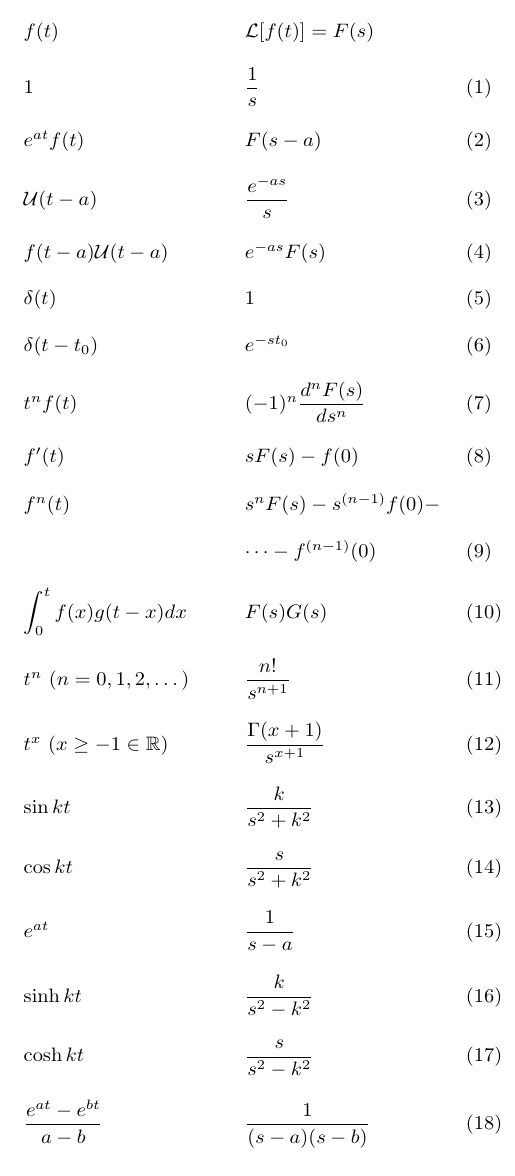
\includegraphics[width=0.98\textwidth]{images/img_koma/laplace_table1.png}\newline
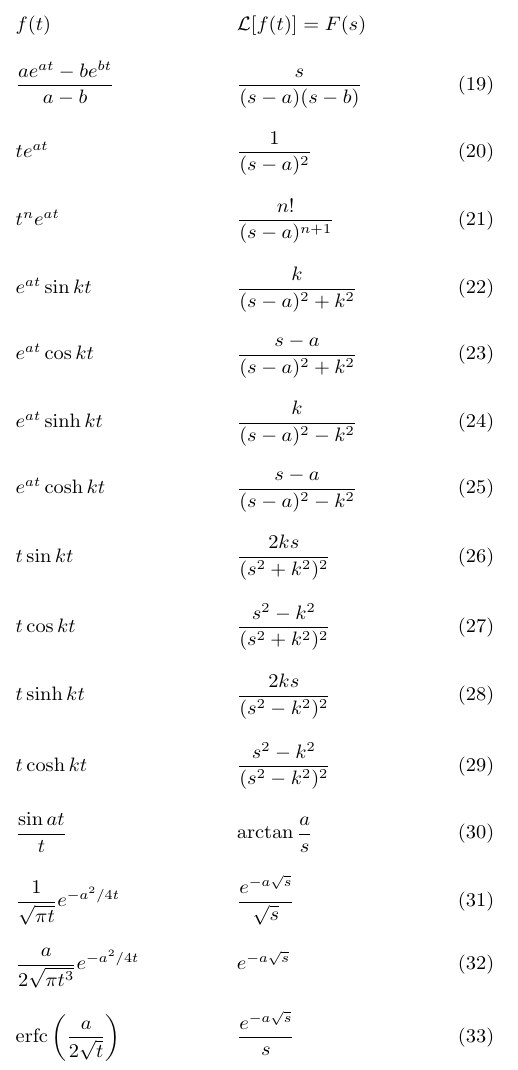
\includegraphics[width=1\textwidth]{images/img_koma/laplace_table2.png}


%\ifx true false
\part{Trigonometrie}
\setcounter{section}{0}

\section{Trigonometrische Definitionen \& Sätze}
\subsection{Definitionen}

$sin(x) := \sum_{n=0}^{\infty} (-1)^n \frac{x^{2n+1}}{(2n+1)!} = \frac{x}{1!} - \frac{x^3}{3!} + \frac{x^5}{5!} \mp ...$

$cos(x) := \sum_{n=0}^{\infty} (-1)^n \frac{x^{2n}}{(2n)!} = \frac{x^0}{0!} - \frac{x^2}{2!} + \frac{x^4}{4!} \mp ...$

$exp(x) := \sum_{n=0}^{\infty} \frac{x^{n}}{n!} = \lim\limits_{n \rightarrow \infty}{(1 + \frac{x^{n}}{n})^n}$

$arctan(x) := \sum_{n=0}^{\infty} (-1)^n \frac{x^{2n+1}}{2n+1} = \frac{x}{1} - \frac{x^3}{3} + \frac{x^5}{5} \mp ...$

Hinweis: Für einfache Approximation genügt es die ersten paar Glieder der $arctan(x)-Reihe$ zu berechnen. \newline 
Falls: $x \notin [0,1]$, gibt es eine Vereinfachung:
$ arctan(x) = \frac{sgn(x) * \pi}{2} - arctan(\frac{1}{x}) $

\subsubsection{Definition Taylorreihe} Eine Funktion $f(x)$ wird an einer Stelle $x_0$ angenähert durch $Tf(x;x_0) = \sum_{n=0}^{\infty} \frac{f^{(n)}(x_0)}{n!}(x - x_0)^n = f(x_0)$ \\

\subsubsection{Definitionen csc(x), sec(x), cot(x)}
$csc(x) := \frac{1}{sin(x)}$ \hfil $sec(x) := \frac{1}{cos(x)}$ \hfil $cot(x) := \frac{1}{tan(x)} = \frac{cos(x)}{sin(x)}$





\subsection{Periodizit"aten}

\begin{minipage}{0.49\linewidth}

\begin{itemize}
	\item \(1\cdot e^{2\pi i k} = 1\) f"ur alle \(k \in \mathbb{Z}\)
	\item	\(e^{\frac{\pi}{2} i k} = i\)
	\item \(e^{-\frac{\pi}{2} i k} = -i\)
	\item \(e^{-2 \pi i k} = 1\)
	\item \(e^{\pi i k} = (-1)^k\)
	\item \(e^{-\pi i k} = (-1)^k\)
\end{itemize}	

\end{minipage}
\hfill
\begin{minipage}{0.49\linewidth}
\begin{itemize}	
	\item $ \sin(z+2 \pi) = \sin(z) $
	\item $ \cos(z+2 \pi) = \cos(z) $
	\item $\sinh(z + 2 \pi i) = \sinh(z)$
	\item $\cosh(z + 2 \pi i) = \cosh(z)$
	\item $ \sin(z- \pi) = -\sin(z) $
	\item $ \cos(z- \frac{\pi}{2}) = \sin(z) $
\end{itemize}
\end{minipage}
\subsection{Winkel}
\renewcommand{\arraystretch}{1.5}
\begin{tabular}{|c|c|c|c|c|c|c|c|c|}
	\hline
	\(\varphi \) &$0$ & \(\frac{\pi}{6}\) & \(\frac{\pi}{4}\) & \(\frac{\pi}{3}\) &  \(\frac{\pi}{2}\) &  \(\frac{2\pi}{3}\) &  \(\frac{3\pi}{4}\) & \(\frac{5\pi}{6}\) \\
	\hline
	Grad & $0^\circ$ & $30^\circ$ & $45^\circ$ & $60^\circ$ & $90^\circ$ & $ 120^\circ$ & $135^\circ$ & $150^\circ$\\
	\hline
	\(\sin(\varphi)\) & $0$ & \(\frac{1}{2}\) & \(\frac{\sqrt{2}}{2}\) & \(\frac{\sqrt{3}}{2}\) & $1$ &  \(\frac{\sqrt{3}}{2}\) &  \(\frac{1}{\sqrt{2}}\) &  \(\frac{1}{2}\)   \\
	\hline
	\(\cos(\varphi)\) &$1$ & \(\frac{\sqrt{3}}{2}\) & \(\frac{\sqrt{2}}{2}\) & \(\frac{1}{2}\) & $0$ & $-\dfrac{1}{2}$ & \(-\frac{1}{\sqrt{2}}\) &  \(-\frac{\sqrt{3}}{2}\)  \\
	\hline
	\(\tan(\varphi)\) &$ 0$ & \(\frac{1}{\sqrt{3}}\) &  $1$ & $\sqrt{3}$ & $\pm \infty$ &$-\sqrt{3}$ & $-1$ &  \(-\frac{1}{\sqrt{3}}\)\\ 
	\hline
\end{tabular}\\

\begin{tabular}{|c|c|c|c|c|c|c|c|}
	\hline
	\(\varphi \) &$\pi$ & \(\frac{7\pi}{6}\) & \(\frac{5\pi}{4}\) & \(\frac{4\pi}{3}\) &  \(\frac{3\pi}{2}\) &  \(\frac{5\pi}{3}\) &  \(\frac{7\pi}{4}\)  \\
	\hline
	Grad & $180^\circ$ & $210^\circ$ & $225^\circ$ & $240^\circ$ & $270^\circ$ & $ 300^\circ$ & $315^\circ$\\
	\hline
	\(\sin(\varphi)\) & $0$ & \(-\frac{1}{2}\) & \(-\frac{\sqrt{2}}{2}\) & \(-\frac{\sqrt{3}}{2}\) & $-1$ &  \(-\frac{\sqrt{3}}{2}\) &  \(-\frac{1}{\sqrt{2}}\)  \\
	\hline
	\(\cos(\varphi)\) &$-1$ & \(-\frac{\sqrt{3}}{2}\) & \(-\frac{\sqrt{2}}{2}\) & \(-\frac{1}{2}\) & $0$ & $\dfrac{1}{2}$ & \(\frac{1}{\sqrt{2}}\)  \\
	\hline
	\(\tan(\varphi)\) &$ 0$ & \(\frac{1}{\sqrt{3}}\) &  $1$ & $\sqrt{3}$ & $\pm \infty$ &$-\sqrt{3}$ & $-1$ \\ 
	\hline
\end{tabular}\\
\renewcommand{\arraystretch}{1.0}

\newpage
\subsection{Sinusssatz}
\begin{figure}[h!]
\centering
    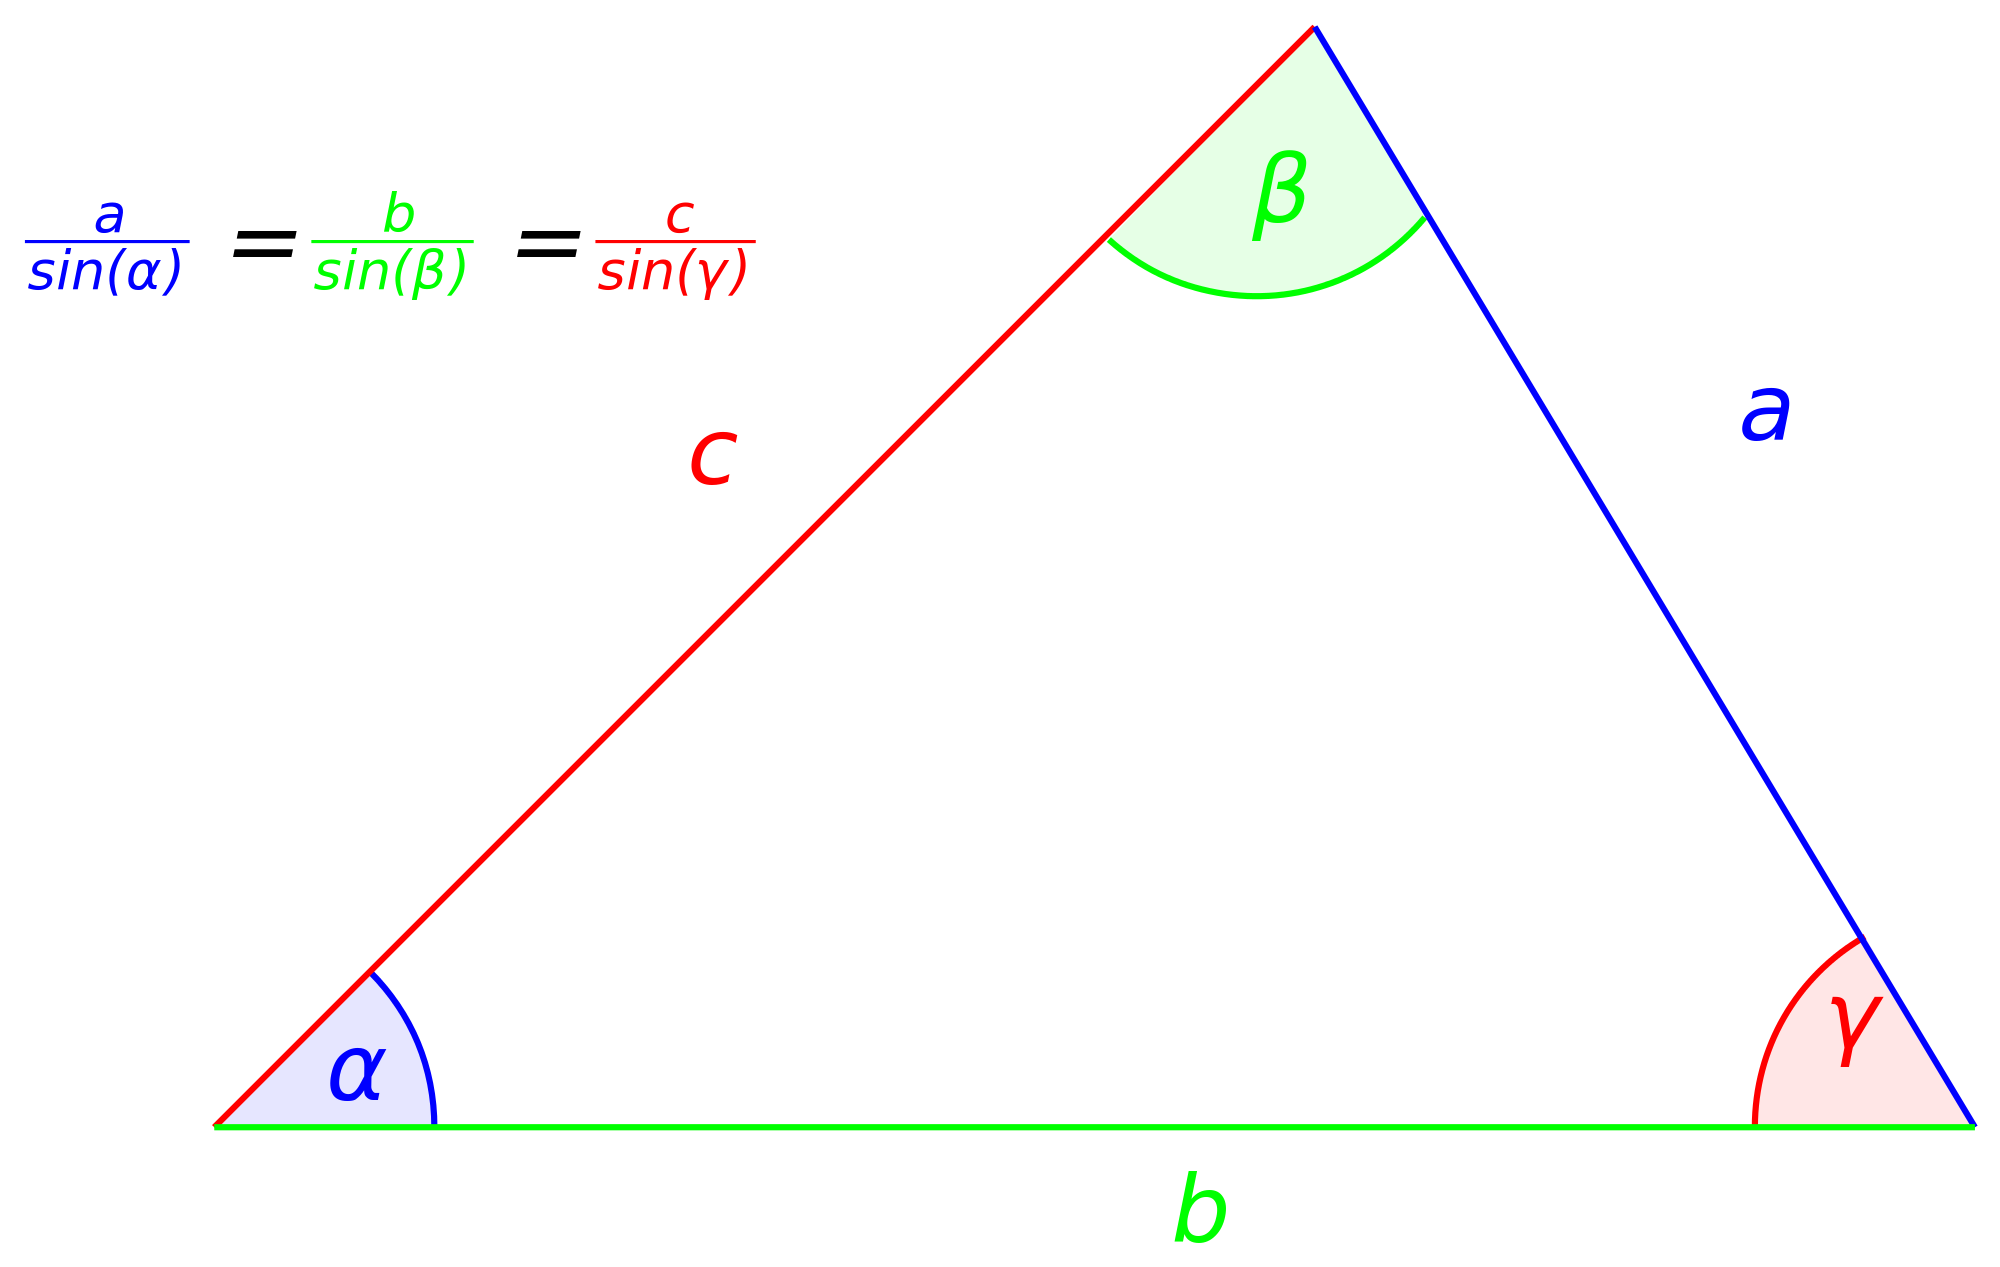
\includegraphics[width=0.5\textwidth]{images/sinussatz.png}
    \caption{Quelle: https://de.wikipedia.org/}
    
\end{figure}
\subsection{Cosinusssatz}
$a^2 + b^2 -2ab*cos(\gamma)= c^2$


\subsection{Standardintegrale}
\begin{minipage}{0.49\linewidth}
$\frac{d}{dx} arcsin(x) = \frac{1}{\sqrt{1-x^2}}$ \\
$\frac{d}{dx} arccos(x) = \frac{-1}{\sqrt{1-x^2}}$ \\
$\frac{d}{dx} arctan(x) =\frac {1}{x^2+1}$ \\
\end{minipage}
\begin{minipage}{0.49\linewidth}
$\frac{d}{dx} arsinh(x) =\frac{1}{\sqrt{x^2+1}}$ \\
$\frac{d}{dx} arcosh(x) =\frac{1}{\sqrt{x^2-1}}, $wenn $ x>1$ \\
$\frac{d}{dx} artanh(x) =\frac{1}{1-x^2}, $wenn $ |x|<1$ \\
\end{minipage}

\subsection{Euler Formel}
$exp(i \phi) = cos(\phi) + isin(\phi)$
\\
$exp(-i \phi) = cos(-\phi) + isin(-\phi) \Longleftrightarrow $ 
$exp(-i \phi) = cos(\phi) - isin(\phi)$ 

Daraus kann nun sin, sinh, cos und cosh in Termen von exp(x) ausgedrückt werden.

$\frac{exp(i \phi) + exp(-i \phi)}{2}  = cos(\phi)$\\
$\frac{exp(i \phi) - exp(-i \phi)}{2i}  = sin(\phi)$

Ignoriere alle i, dann folgt...

$\frac{exp(\phi) + exp(-\phi)}{2}  = cosh(\phi)$\\
$\frac{exp(\phi) - exp(-\phi)}{2}  = sinh(\phi)$




\subsection{Ableitungen, Integrale}
\subsection{Ableitungen}
$\frac{d}{dx}sin(x) = cos(x)$

$\frac{d}{dx}cos(x) = -sin(x)$

$\frac{d}{dx}tan(x) = \frac{d}{dx} \frac{sin(x)}{cos(x)} = \frac{cos(x)cos(x)- sin(x)sin(x)}{cos^2(x)} = 1 - \frac{sin^2(x)}{cos^2(x)} = 1 - tan^2(x) = \frac{1}{cos^2(x)}$

$\frac{d}{dx} \frac{1}{sin(x)} = \frac{0*sin(x) - 1*cos(x)}{sin^2(x)} = \frac{-cos(x)}{sin^2(x)}$ 

$\frac{d}{dx} \frac{1}{cos(x)} = \frac{0*cos(x) - 1*(-sin(x))}{cos^2(x)} = \frac{sin(x)}{cos^2(x)}$

$\frac{d}{dx}sin^2(x) = sin(x)*cos(x)+ cos(x)*sin(x) = 2*sin(x)*cos(x)$

$\frac{d}{dx}cos^2(x) = cos(x)*(-sin)(x)+ (-sin(x))*cos(x) = -2*sin(x)*cos(x)$ 
\newpage
\subsection{Rechenregeln}
\subsection{Additionstheoreme}
$sin^2(x)+cos^2(x) = 1$

$sin(x \pm y) = sin(x)cos(y) \pm cos(x)sin(y)$    \ \ $(\# umgekehrteAbleitungsregel)$

$cos(x \pm y) = cos(x)cos(y) \mp \sinx \siny$

$tan(x \pm y) = \frac{\tanx \pm \tany}{ 1 \mp \tanx \; \tany } = \frac{ sin(x \pm y) }{cos(x \pm y) }$

\subsection{Doppelwinkel}
$sin(2x)= 2\sinx \cosx = \frac{2 \tanx}{ 1 + tan^2(x) }$

$cos(2x)= cos^2(x) - sin^2(x) = 1 - 2sin^2(x) = 2cos^2(x) - 1 = \frac{ 1 - tan^2(x) }{ 1 + tan^2(x) }$

$tan(2x)= \frac{ 2 \tanx }{ 1 - tan^2(x) } = \frac{2}{ cot(x) - \tanx }$

$cot(2x)= \frac{ cot^2(x) - 1}{2cot(x)} = \frac{cot(x) - \tanx}{2}$ \\

Beweis mit Additionstheorem



\subsection{Produkt-zu-Summen-Formel}
$\sinx*sin(y) = \frac{1}{2}(cos(x-y)-cos(x+y))$

$\cosx*cos(y) = \frac{1}{2}(cos(x-y)+cos(x+y))$

$sin(x)*cos(y) = \frac{1}{2}(sin(x-y)+sin(x+y))$ \\



\subsection{Hyperbolische Funktionen}
$sinh(z) := \frac{e^z - e^{-z}}{2} = z + \frac{z^3}{3!} + \frac{z^5}{5!} + \frac{z^7}{7!} + \dots = \sum_{n=0}^\infty \frac{z^{2n+1}}{(2n+1)!}$

$cosh(z) := \frac{e^z + e^{-z}}{2}= 1 + \frac{z^2}{2!} + \frac{z^4}{4!} + \frac{z^6}{6!} + \dots = \sum_{n=0}^\infty \frac{z^{2n}}{(2n)!}$

$sin(z)= Im(e^{iz})=\dfrac{1}{2i} (e^{iz}-e^{-iz})$ \\

$cos(z)=\text{Re}(e^{iz})=\dfrac{1}{2}(e^{iz}+e^{-iz})$ \\

$sinh(\pm iz) = \pm i \cdot \sin(z)$\\
$cosh(\pm iz) = cos(z)$\\
$sin(iz)= i\cdot sinh(z)$\\
$cos(iz)=cosh(z)$\\

$ \sin(-z) = - \sin(z) $\\
$ \tan-(z) = -\tan(z) $\\
$ \cos(-z) = \cos(z) $ \\
$ \arctan(-z) = -\arctan(z) $

$\sin(z) = \sin(x)\cosh(y) + i\cos(x)\sinh(y)$\\
$\cos(z) = \cos(x)\cosh(y) - i\sin(x)\sinh(y)$\\
$e^z = e^x \cos(y) + i e^x \sin(y)$\\
$\sinh(z) = \cos(y)\sinh(x) + i\sin(y)\cosh(x)$\\
$\cosh(z) = \cos(y)\cosh(x) + i\sin(y)\sinh(x)$	

\begin{itemize}[leftmargin=*]
	\item $\int \sinh(ax + b) \,dx = \frac{\cosh(ax + b)}{a}$; $\int \sinh(x) \,dx
	= \cosh(x)$
	\item $\int \cosh(ax + b) \,dx = \frac{\sinh(ax + b)}{a}$; $\int \cosh(x) \,dx
	= \sinh(x)$
	\item $\int \tan(ax + b) \,dx = \frac{\log(\cosh(ax+b))}{a}$; $\int \tan(x)
	\,dx = \log(\cosh(x))$
\end{itemize}


\subsection{Additionstheoreme}
$sinh(z_1 \pm z_2) = sinh(z_1) \cdot cosh(z_2) \pm sinh(z_2) \cdot cosh(z_1)$

$cosh(z_1 \pm z_2) = cosh(z_1) \cdot cosh(z_2) \pm sinh(z_1) \cdot sinh(z_2)$

$tanh(z_1 \pm z_2) = \frac{tanh(z_1) \pm tanh(z_2)}{1 \pm tanh(z_1) \cdot tanh(z_2)}$


\subsubsection{Zusammenhänge}
$cosh^2(z) - sinh^2(z) = 1$ \hfill $cosh(z) + sinh(z) = e^z$ \hfill $cosh(z) - sinh(z) = e^{-z}$

\subsection{Ableitungen}
$\frac{d}{dz}sinh(z) = cosh(z)$ \hfill $\frac{d}{dz}cosh(z) = sinh(z)$ \hfill $\frac{d}{dz}tanh(z) = 1 -tanh^2(z) = \frac{1}{cosh^2(x)}$

\section{Plots Trigonometrischer Funktionen}
%Alle Plots in diesem Kapitel von www.wikipedia.org!

\begin{figure}[!htb]
	\centering
	\begin{minipage}{.5\textwidth}
		\centering
		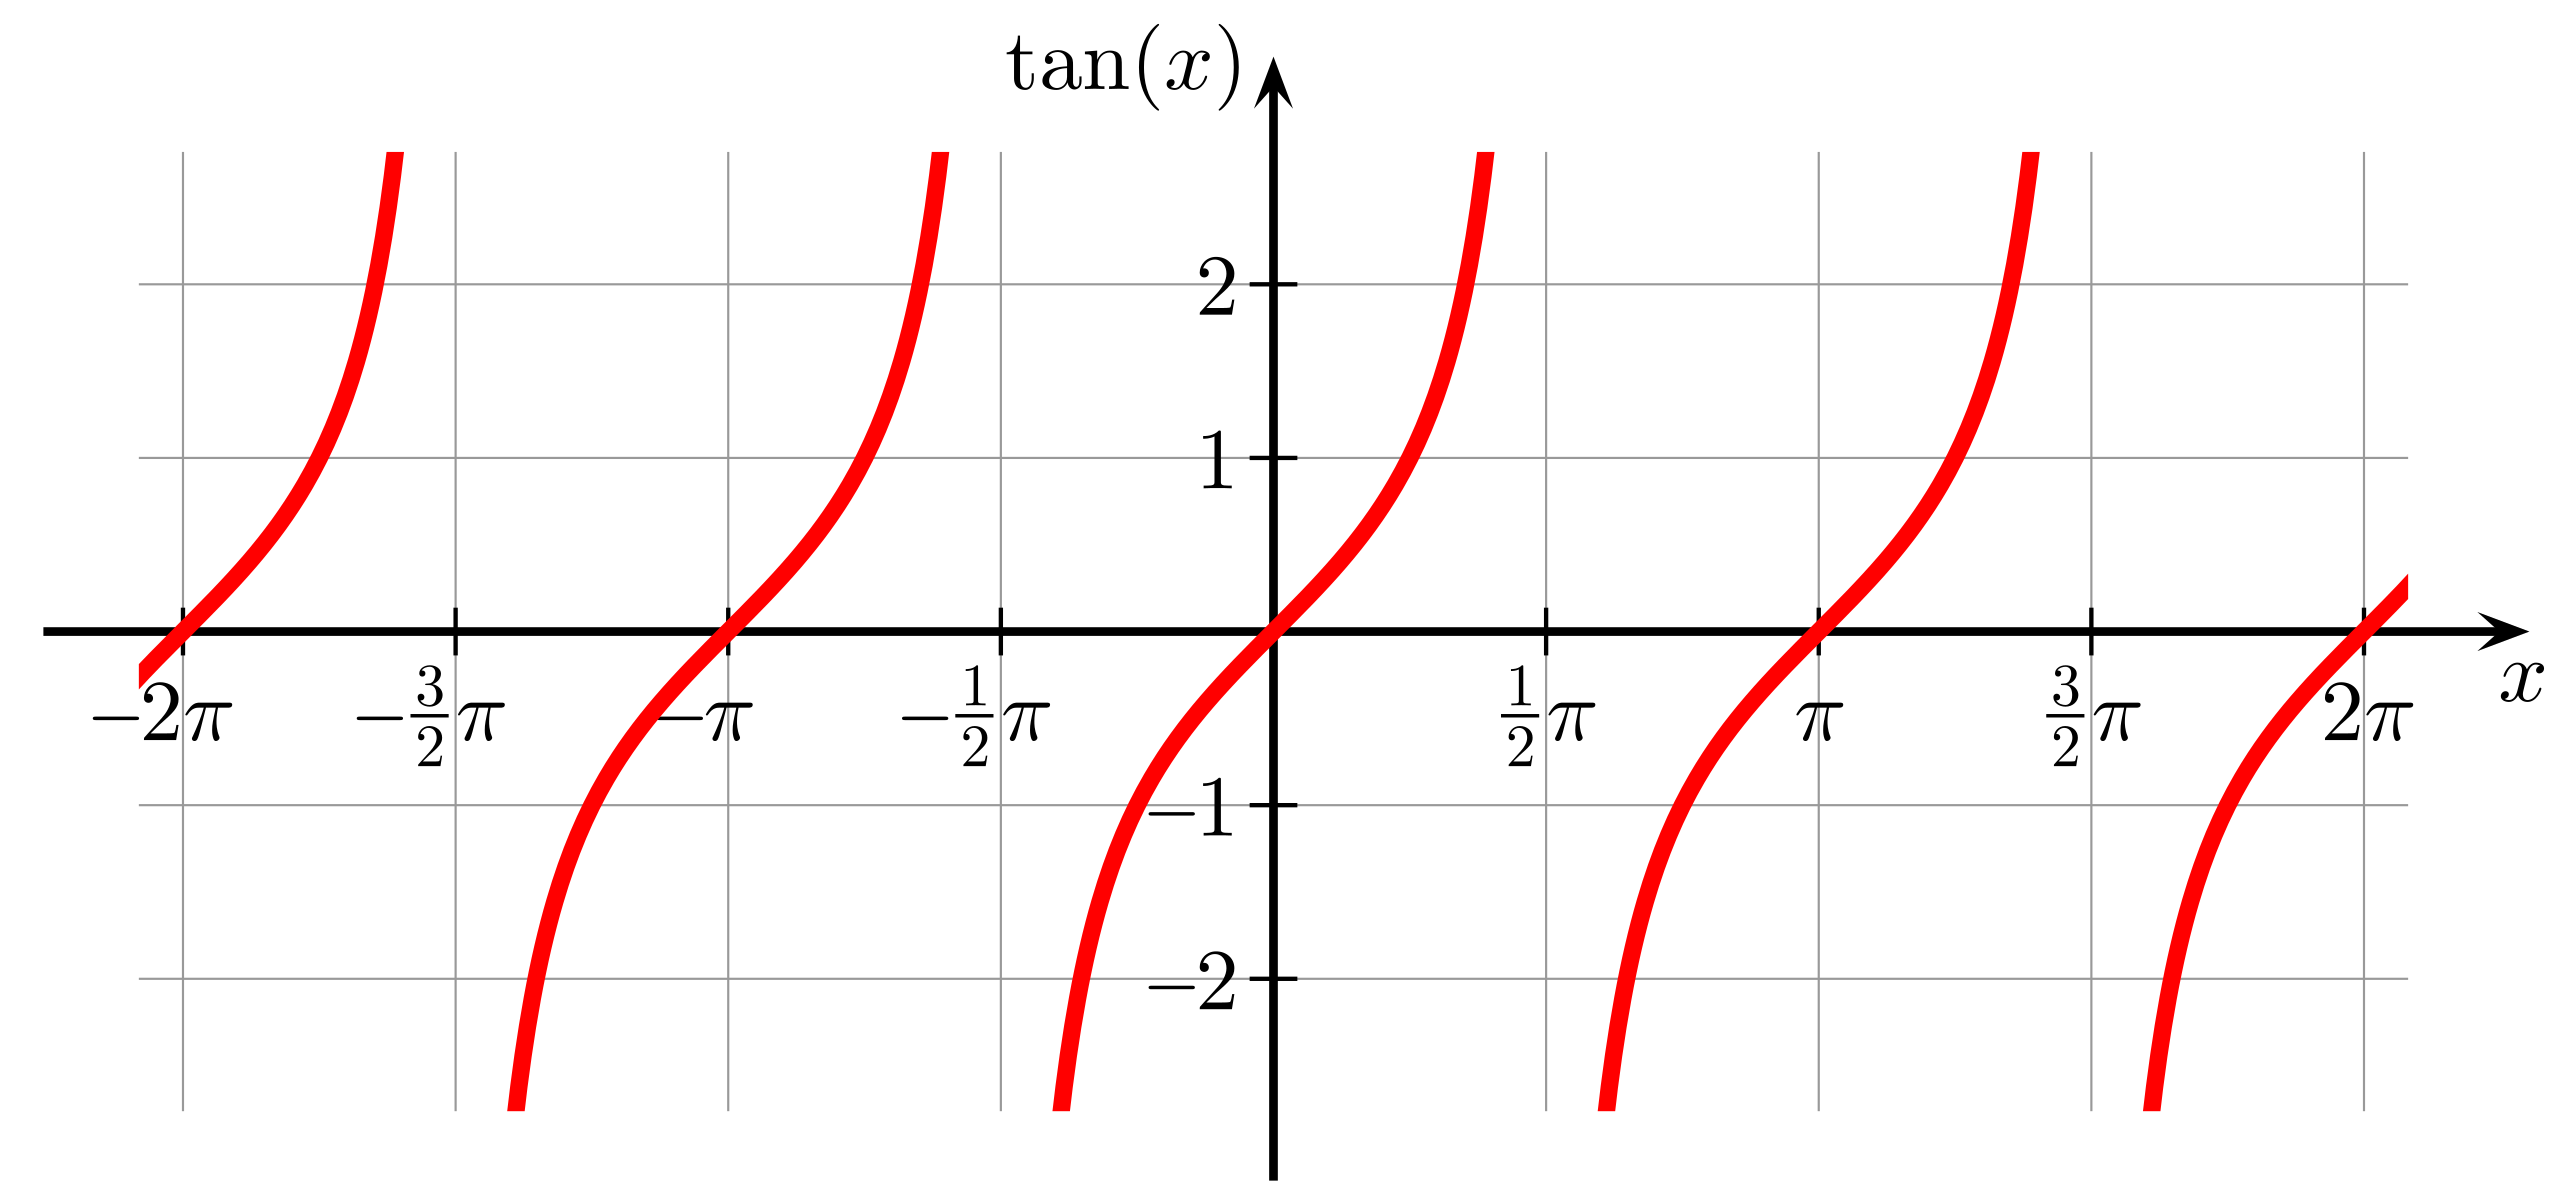
\includegraphics[width=1\linewidth]{images/tan.png}
	\end{minipage}%
	\begin{minipage}{0.5\textwidth}
		\centering
		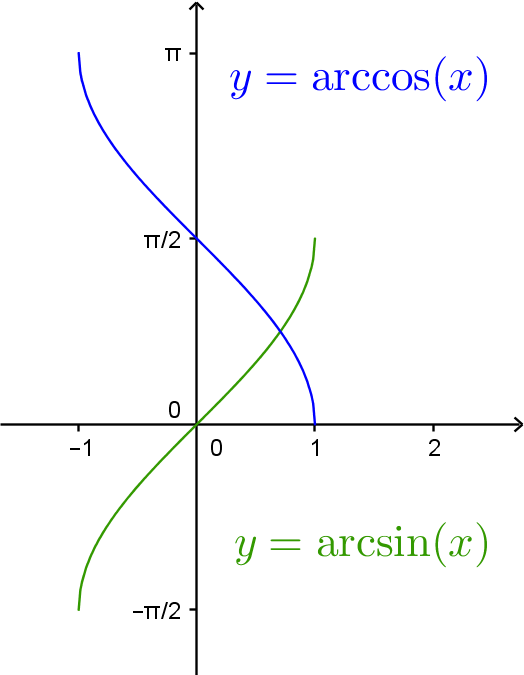
\includegraphics{images/asinacos.png}
	\end{minipage}
\end{figure}


\begin{figure}[H] 
	\centering
	{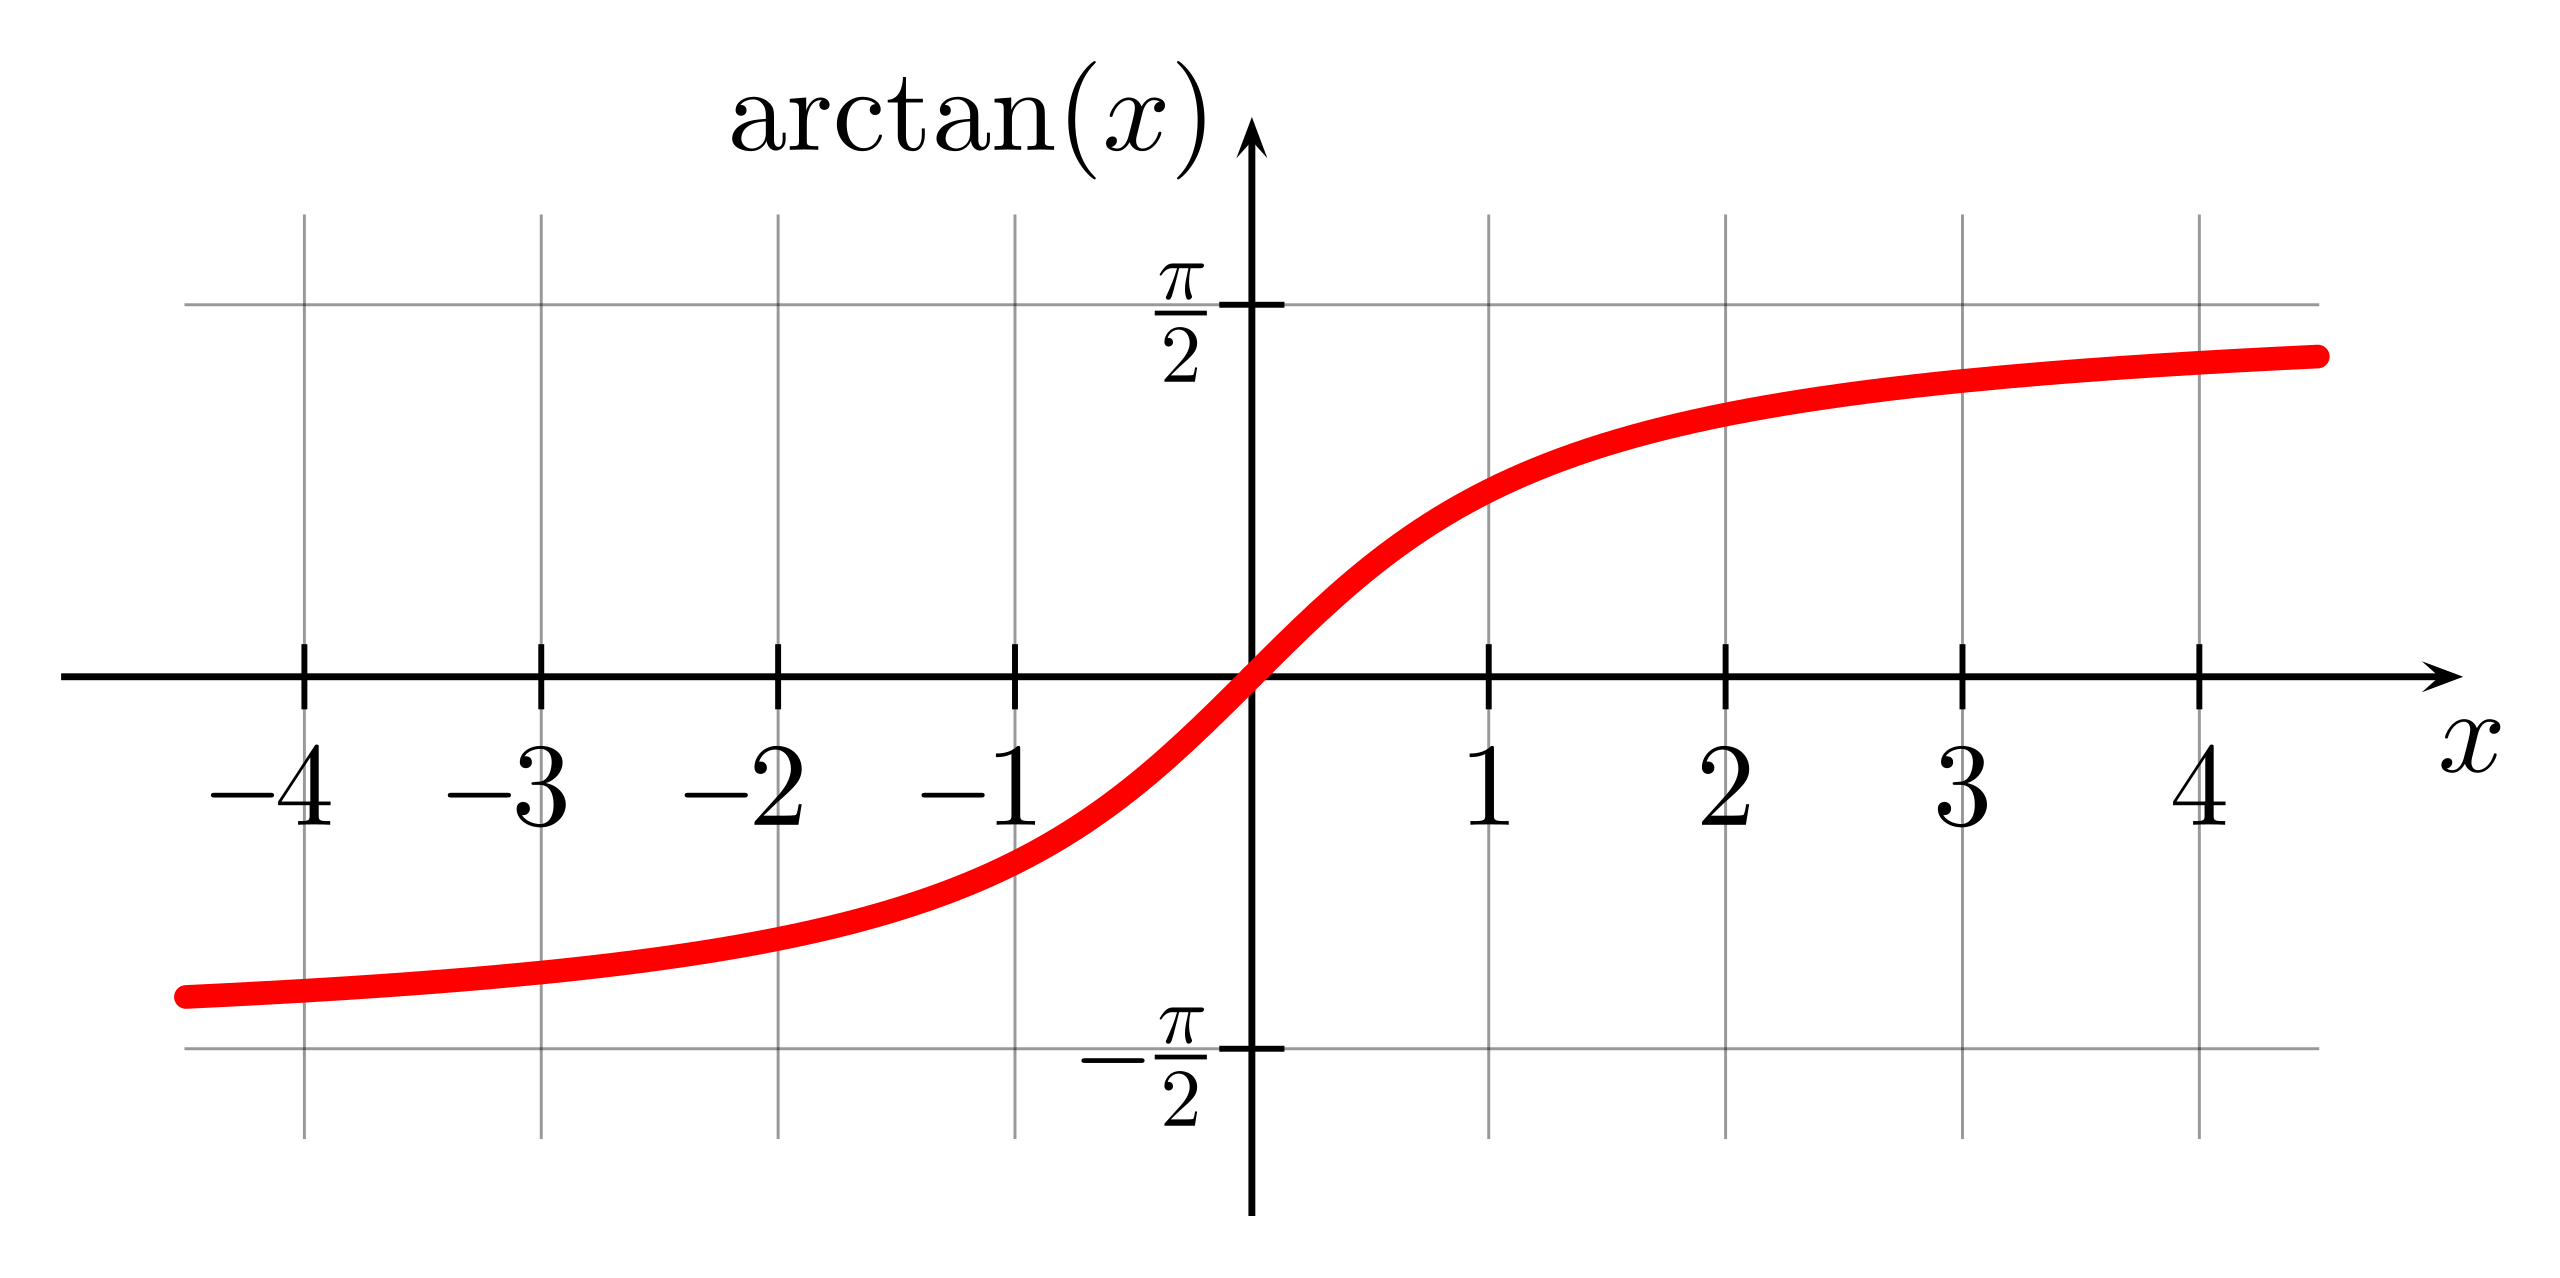
\includegraphics[width=0.55\textwidth]{images/arctan.png}}
\end{figure}



\begin{figure}[!htb]
	\centering
	\begin{minipage}{.5\textwidth}
		\centering
		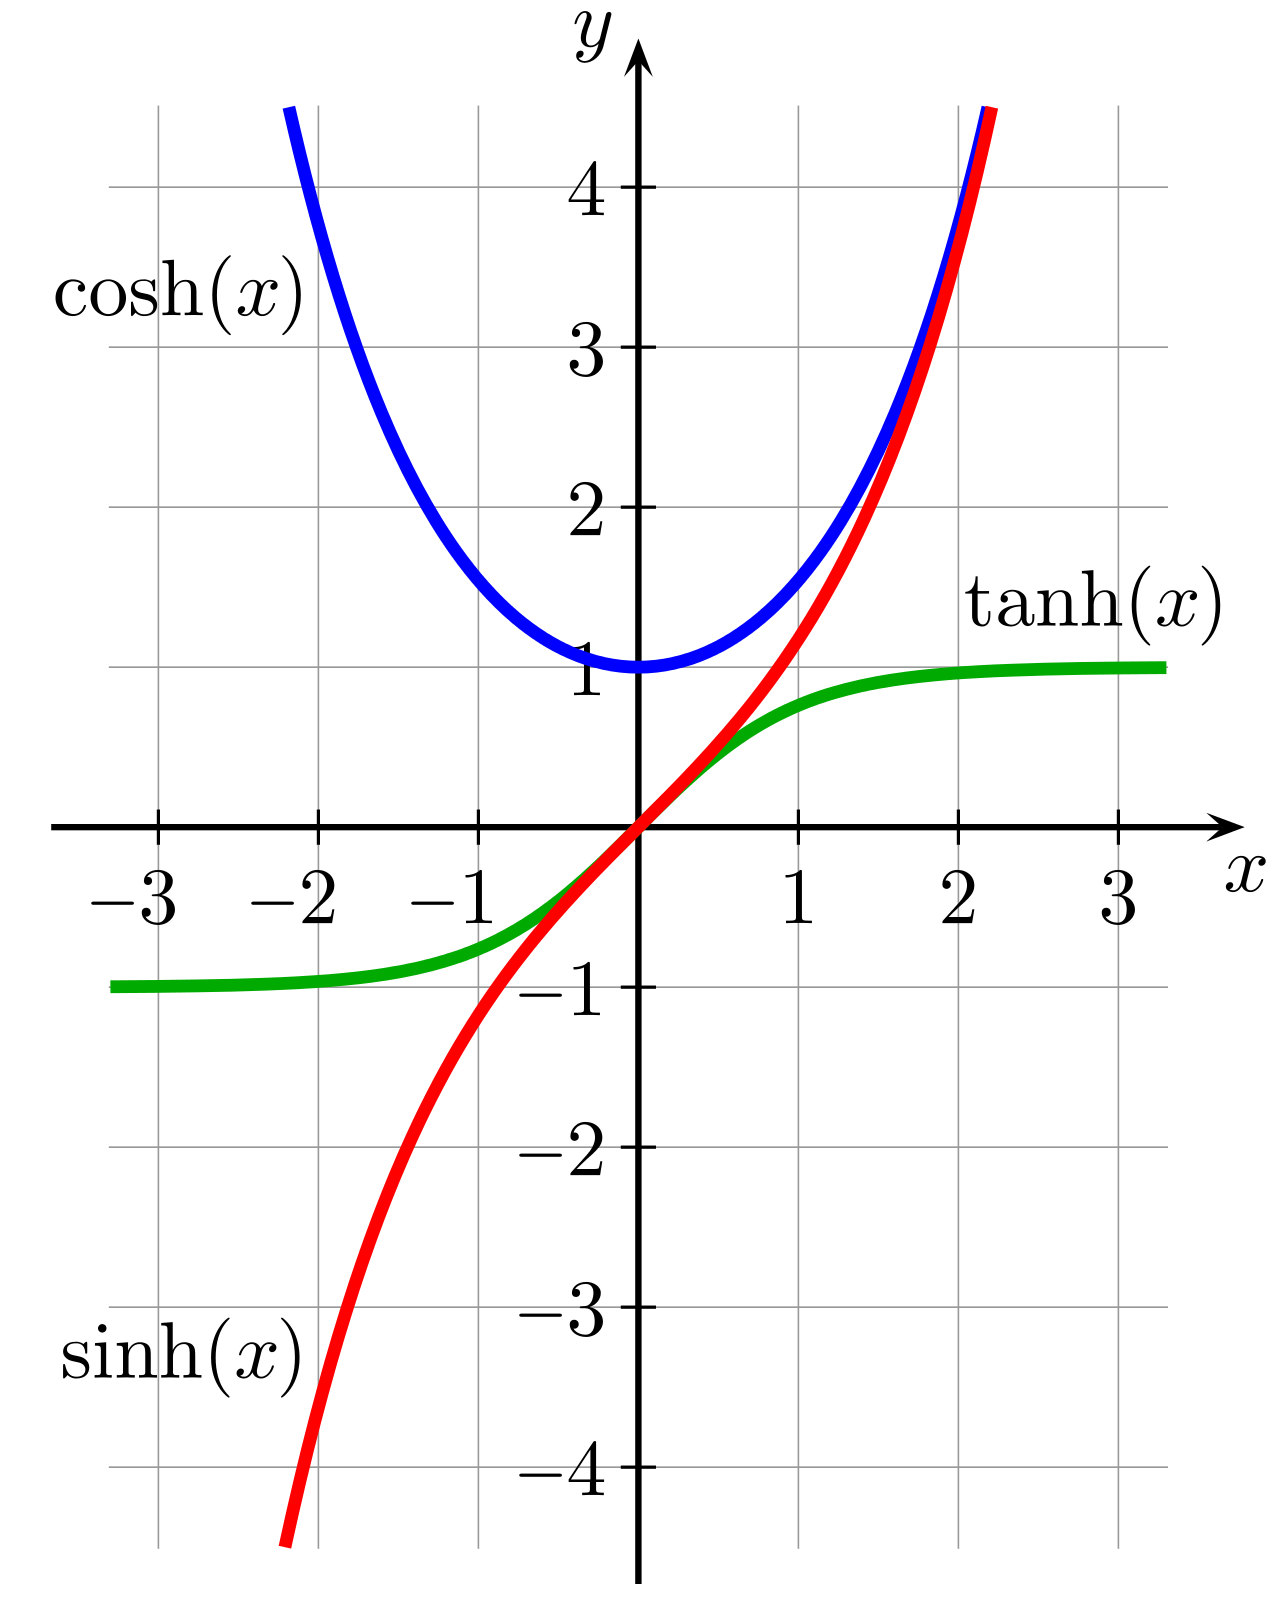
\includegraphics[width=1\linewidth]{images/sinhcoshtanh.png}
	\end{minipage}%
	\begin{minipage}{.5\textwidth}
		\centering
		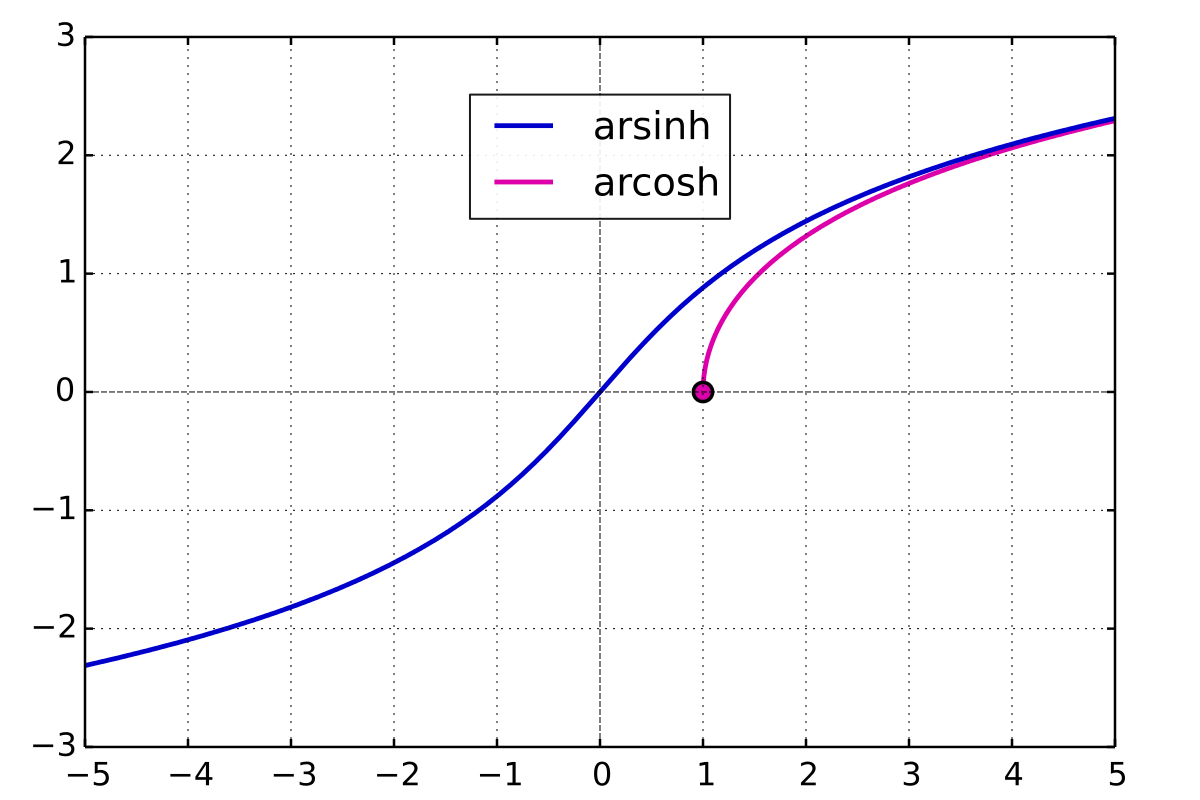
\includegraphics[width=1\linewidth]{images/arsinharcosh.png}
	\end{minipage}
\end{figure}


%

\section{Koordinatensysteme mit Funktionaldeterminante}

\subsection{Polarkoordinaten}
\begin{figure}[h!]
\centering
    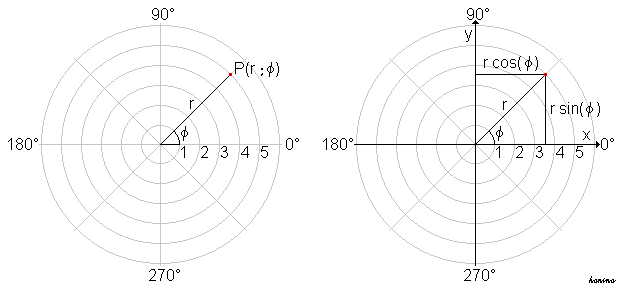
\includegraphics[width=0.6\textwidth]{images/Ebene_polarkoordinaten.PNG}
    \caption{Quelle: https://de.wikipedia.org/}
    
\end{figure}

Umrechnung erfolgt durch: \\
$x=r\cos\varphi$\\
$y=r\sin\varphi$\\

Aus den Umrechnungsformeln von Polarkoordinaten in kartesische Koordinaten erhält man für die Funktionaldeterminante als Determinante der Jacobi-Matrix:\\
\\$
\det J = \det\frac{\partial(x,y)}{\partial(r,\varphi)}
=\begin{vmatrix}
  \frac{\partial x}{\partial r} & \frac{\partial x}{\partial \varphi} \\
  \frac{\partial y}{\partial r} & \frac{\partial y}{\partial \varphi}
\end{vmatrix}
=\begin{vmatrix}
  \cos\varphi & -r\sin\varphi \\
  \sin\varphi &  r\cos\varphi
\end{vmatrix} =r\cos^2\varphi + r\sin^2\varphi = r
$

\subsection{Zylinderkoordinaten}
\begin{figure}[h!]
\centering
    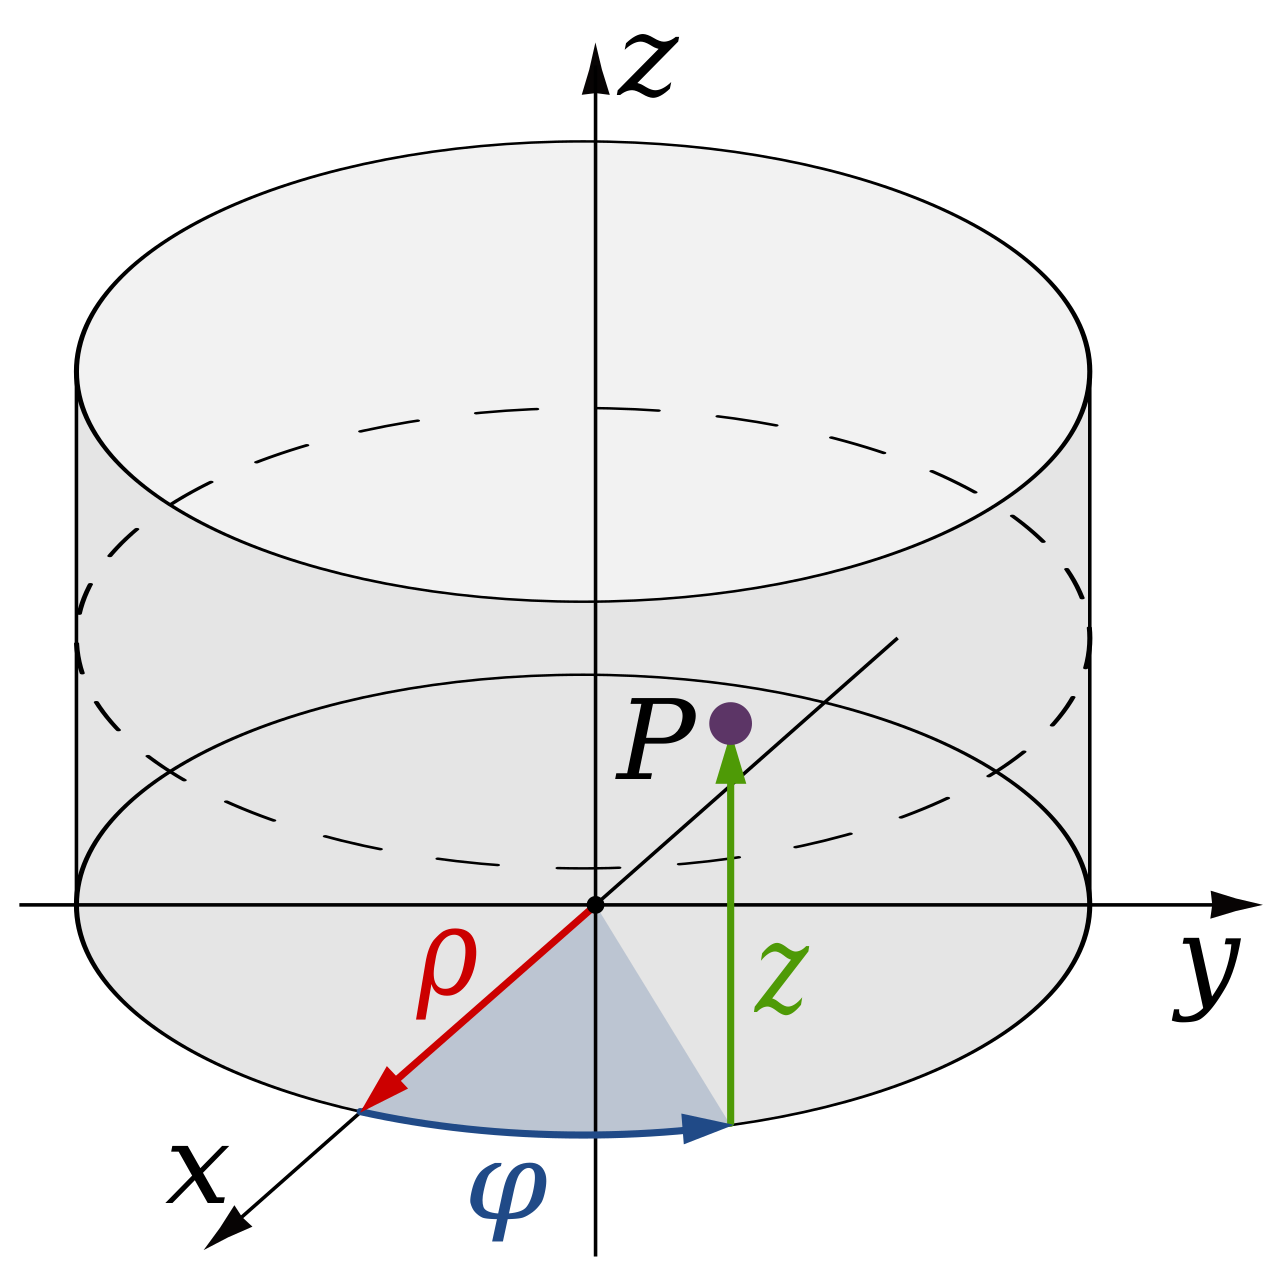
\includegraphics[width=0.3\textwidth]{images/zylinderkoord.png}
    \caption{Quelle: https://de.wikipedia.org/}
    
\end{figure}
Umrechnung erfolgt durch: \\
$x=\rho\ \cos\varphi$\\
$y=\rho\ \sin\varphi$\\
$z=z$\\

Mit Funktionaldeterminante:
$
\det\frac{\partial(x,y,z)}{\partial(\rho,\varphi,z)}=\begin{vmatrix}
  \cos\varphi & -\rho\sin\varphi & 0 \\
  \sin\varphi &  \rho\cos\varphi & 0 \\
            0 &                0 & 1
\end{vmatrix}=\rho$


\subsection{Kugelkoordinaten}
\begin{figure}[h!]
\centering
    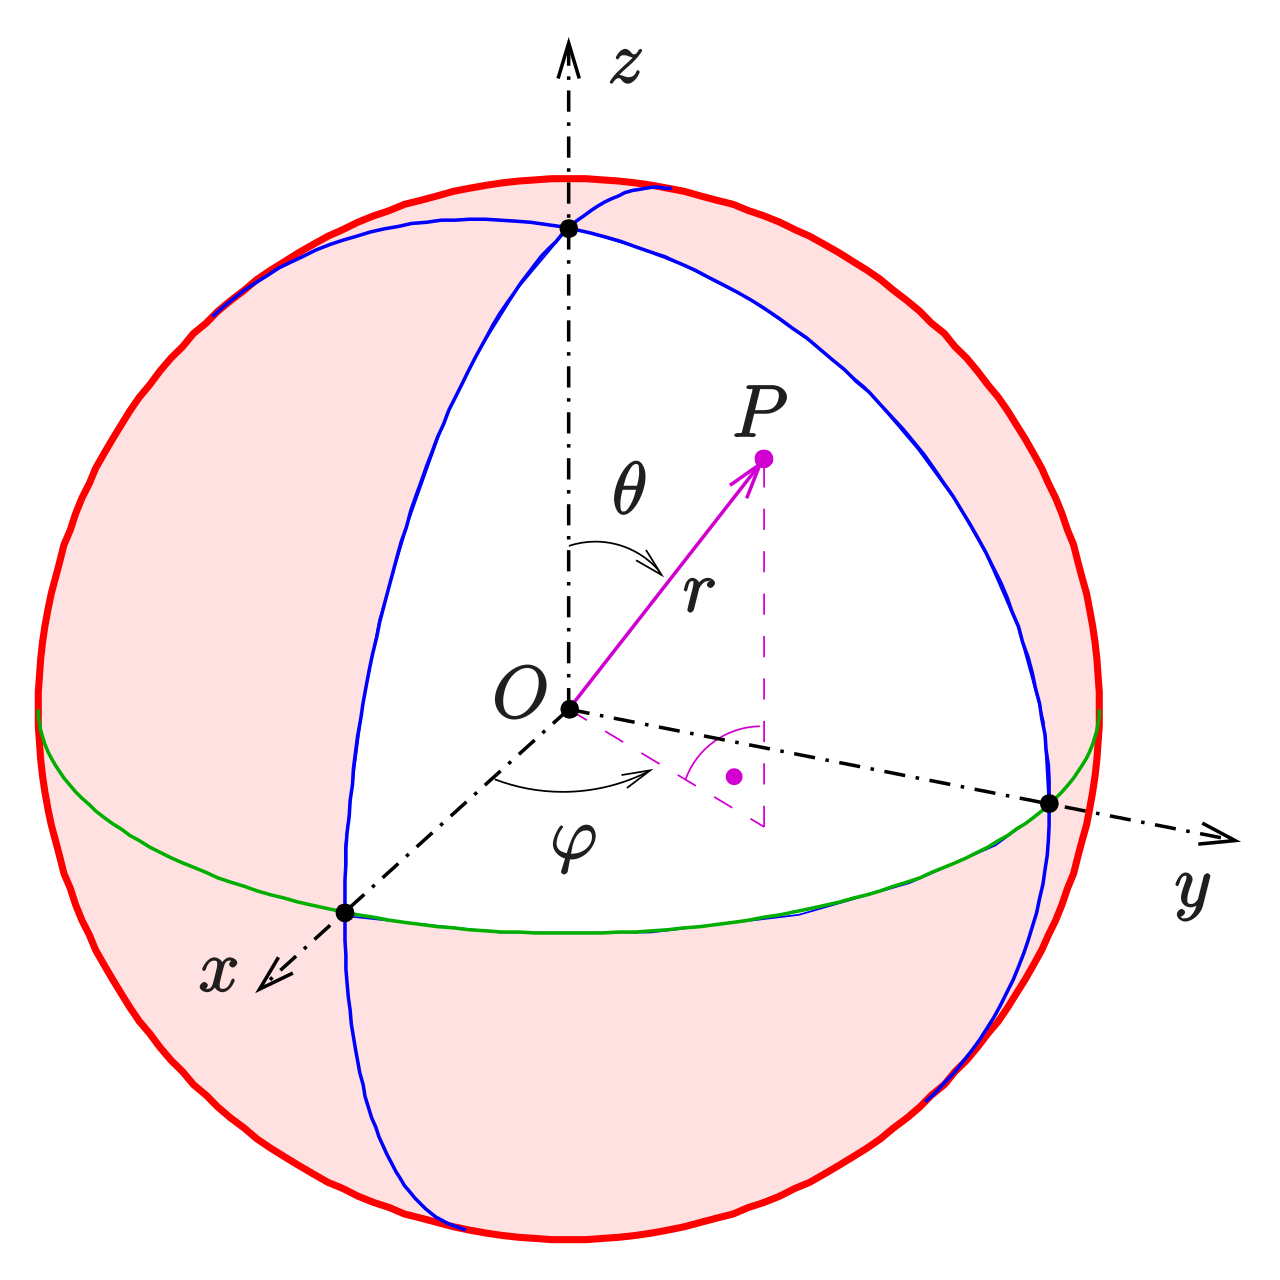
\includegraphics[width=0.4\textwidth]{images/kugelkoord.png}
    \caption{Quelle: https://de.wikipedia.org/}
    
\end{figure}

Umrechnung erfolgt durch: \\
$x = r \cdot \sin \theta \cdot \cos \varphi$ \\
$y = r \cdot \sin \theta \cdot \sin \varphi$ \\
$z = r \cdot \cos \theta$ \\

Jacobi-Matrix:

$J =\frac{\partial(x,y,z)}{\partial(r,\theta,\varphi)}
  =\begin{pmatrix}
     \sin\theta\cos\varphi&r\cos\theta\cos\varphi&-r\sin\theta\sin\varphi\\
     \sin\theta \sin\varphi&r\cos\theta\sin\varphi&r\sin\theta\cos\varphi\\
     \cos\theta&-r\sin\theta&0
   \end{pmatrix}$\\
   
   mit Funktionaldeterminante:
   $\det J=r^2\sin\theta$








\section{Rotationsmatrix, Drehmatrix}

\subsection{Drehmatrix der Ebene}
Jede Rotation um den Ursprung ist eine lineare Abbildung. Wie bei jeder linearen Abbildung genügt daher zur Festlegung der Gesamtabbildung die Festlegung der Bilder der Elemente einer beliebigen Basis. Wird die Standardbasis gewählt, sind die Bilder der Basisvektoren gerade die Spalten der dazugehörigen Abbildungsmatrix.

Wir haben unter $R_{\alpha}$ \\
\\
 $\begin{pmatrix} 1 \\ 0 \end{pmatrix} \mapsto \begin{pmatrix} \cos\alpha \\ \sin\alpha \end{pmatrix}
\qquad\text{und}\qquad
\begin{pmatrix} 0 \\ 1 \end{pmatrix} \mapsto \begin{pmatrix} -\sin\alpha \\ \cos\alpha \end{pmatrix}$ \newline

Die Drehmatrix für eine Drehung um $\alpha$ ist also:  \newline
$R_\alpha = \begin{pmatrix} \cos\alpha & -\sin\alpha \\ \sin\alpha & \newline \cos\alpha\end{pmatrix}$

 $\begin{pmatrix} x' \\ y' \end{pmatrix} = \begin{pmatrix} \cos\alpha & -\sin\alpha \\ \sin\alpha & \cos\alpha\end{pmatrix} \cdot \begin{pmatrix} x \\y \end{pmatrix}$\\

\subsubsection{Herleitung}
\begin{figure}[H] 
\centering
    {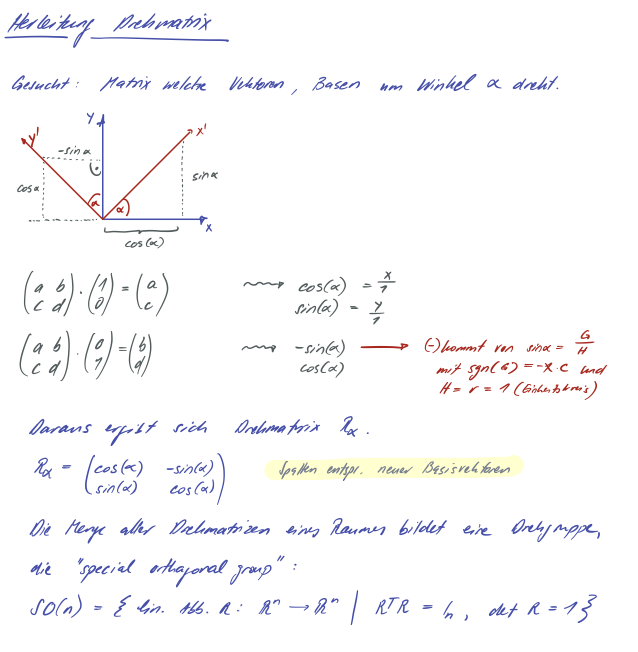
\includegraphics[width=0.75\textwidth]{images/herldrehmat.png}}
    \caption{Quelle: Miles Strässle, 20.11.2019}    
\end{figure}

\subsection{Drehmatrix in 3-Dimensionen}
In der Physik werden häufig Drehungen des Koordinatensystems benutzt, dann müssen bei den untenstehenden Matrizen die Vorzeichen aller Sinus-Einträge vertauscht werden. Die Drehung eines Vektors um einen bestimmten Winkel in einem Koordinatensystem ist äquivalent zur Drehung des Koordinatensystems um den gleichen Winkel in umgekehrter Richtung (Drehung um negativen Winkel). 
\vspace{0.5cm}
„Der Drehsinn ergibt sich, wenn man entgegen der positiven Drehachse auf den Ursprung sieht.“

\subsubsection{Drehung um die x-Achse:}
$R_x(\alpha) = \begin{pmatrix}
1 &   0         & 0           \\
0 & \cos \alpha & -\sin \alpha \\
0 & \sin \alpha &  \cos \alpha
\end{pmatrix}$
\subsubsection{Drehung um die y-Achse:}
$R_y(\alpha) = \begin{pmatrix}
\cos \alpha  & 0 & \sin \alpha \\
   0         & 1 &  0          \\
-\sin \alpha & 0 & \cos \alpha
\end{pmatrix}$
\subsubsection{Drehung um die z-Achse:}
$R_z(\alpha) = \begin{pmatrix}
\cos \alpha & -\sin \alpha & 0 \\
\sin \alpha &  \cos \alpha & 0 \\
   0        &  0           & 1
\end{pmatrix}$


 %additional Koordinatensysteme und Drehmatrixen inkl. Herleitung
\part{Differenzialrechnung}
\setcounter{section}{0}

\section{Differentialgleichungen}

\subsection{Grundbegriffe}

\begin{description}[labelindent=16pt,style=multiline,leftmargin=3.5cm, noitemsep]
	\item[Ordnung:] h{\"o}chste vorkommende Ableitung
	\item[linear:] alle $y$-abh{\"a}ngigen Terme kommen linear vor (keine Terme wie zum Beispiel $y^2$, $(y'')^3$, $\sin(y)$, $e^{y'}$)
	\item[homogen:] Gleichung ohne St{\"o}rfunktionen
	\item[St{\"o}rfunktion:] Term, der rein von der Funktionsvariablen $x$ abh{\"a}ngt
\end{description}

\subsection{Methoden}

\begin{table}[H]
	\centering
	\begin{tabular}{|p{3cm}|p{6cm}|p{3cm}|}
		\hline
		& \textbf{Problem} 							& \textbf{Anforderungen} 			\\ \hline
		\textbf{Trennung der Variablen}   	& $y' = \frac{dy}{dx} = h(x) \cdot g(y)$ 	& 1. Ordnung			            \\ \hline
		\textbf{Variation der Konstanten}	& $y' = \frac{dy}{dx} = h(x)y + b(x)$	 	& 1. Ordnung \filbreak inhomogen	\\ \hline
		\textbf{Euler-Ansatz}				& $a_{n}y^{(n)} + a_{n-1}y^{(n-1)} + ... + a_{0}y = 0$	 	& n. Ordnung \filbreak linear \filbreak homogen	\\ \hline
		\textbf{Direkter Ansatz}				& $a_{n}y^{(n)} + a_{n-1}y^{(n-1)} + ... + a_{0}y = b(x)$	& n. Ordnung \filbreak linear \filbreak inhomogen	\\ \hline
		
		%\textbf{Substitution}				& $y' = h(\frac{y}{x})$ \filbreak $y' = h(ax + by + c)$ \filbreak $y' = h(\frac{ax + by + c}{dx + ey + f})$ \filbreak $y' = \frac{y}{x}h(xy)$ 																		& nicht direkt separierbar			\\ \hline
	\end{tabular}
\end{table}

\subsubsection{Trennung der Variable}

\begin{equation*}
\begin{split}
& y' + x \tan y = 0,\ y(0) = \frac{\pi}{2} \\
\text{umformen}\quad & \frac{dy}{dx} = -x \tan y \\
\textbf{konstante L{\"o}sungen}\quad & y(x) \equiv 0\ \text{erf{\"u}llt jedoch $y(0) \equiv \frac{\pi}{2}$ nicht} \\
\text{Trennung}\quad & \frac{dy}{\tan y} = -x dx \\
\text{integrieren}\quad & \int\frac{\cos y}{\sin y}dy = - \int xdx \Rightarrow \log|\sin y| = -\frac{x^2}{2} + C \\
& \Rightarrow |\sin y| = e^Ce^{\frac{-x^2}{2}} \Rightarrow \sin y = \pm e^Ce^{\frac{-x^2}{2}} = Ce^{\frac{-x^2}{2}} \\
\text{Anfangsbedingung gebrauchen}\quad & \sin(y(0)) = \sin (\frac{\pi}{2}) = 1 \Rightarrow C = 1 \\
\textbf{L{\"o}sung}\quad & y(x) = \arcsin (e^{\frac{-x^2}{2}})
\end{split}
\end{equation*}

\clearpage

\subsubsection{Variation der Konstanten}

\begin{equation*}
\textbf{Grundsatz:}\quad y(x) = y_h(x) + y_p(x)
\end{equation*}

\begin{equation*}
\begin{split}
& y'(x+1) + y = x^3,\ y(0) = \sqrt{5} \\
\text{Trennung}\quad & \frac{y'}{y} = \frac{-1}{x+1} \\
\textbf{konstante L{\"o}sungen}\quad & y(x) \equiv 0\ \text{erf{\"u}llt jedoch $y(0) \equiv \sqrt{5}$ nicht} \\
\text{integrieren}\quad & \int \frac{dy}{y} = - \int \frac{dx}{x+1} \\
& \Rightarrow \ln|y| = -\ln|x+1| + C \\
\textbf{Homogene L{\"o}sung} \quad & y_h(x) = \frac{C}{x+1},\ \text{mit}\ C= \pm e^C \in \mathbb{R}\backslash{0} \\
\text{partikul{\"a}rer Ansatz}\quad & y_p(x) = \frac{C(x)}{x+1} \\
\text{einsetzen} \quad & (\frac{C'(x)}{x+1} - \frac{C(x)}{(x+1)^2})(x+1) + \frac{C(x)}{x+1} = x^3 \\
& C'(x) = x^3 \\
& C(x) = \frac{x^4}{4} \\
\textbf{partkul{\"a}re L{\"o}sung} \quad & y_p(x) = \frac{x^4}{4(x+1)} \\
\text{allgemeine L{\"o}sung}\quad & y(x) = y_h(x) + y_p(x) = \frac{C}{x+1} + \frac{x^4}{4(x+1)} \\
\text{Anfangsbedingung benutzen} \quad & y(0) = \sqrt{5} \Rightarrow C = \sqrt{5} \\
\textbf{L{\"o}sung} \quad & y(x) = \frac{\sqrt{5}}{x+1} + \frac{x^4}{4(x+1)}
\end{split}
\end{equation*}

%\subsubsection{Substitution}
%
%\begin{equation*}
%\begin{split}
%	& y' = h(\frac{y}{x})\ \text{ersetzt durch}\ z(x) = \frac{y(x)}{x} \Leftrightarrow y(x) = xz(x) \\
%	& \Rightarrow	y' = z + xz'
%\end{split}
%\end{equation*}



\subsubsection{Euler-Ansatz}

\begin{equation*}
\begin{split}
& y'' - 2y' - 8y = 0,\ y(1) = 1, y'(1) = 0 \\
\text{Euler-Ansatz}\quad & y(x) = e^{\lambda x} \\
\text{einsetzen}\quad & \lambda^2 e^{\lambda x} - 2\lambda e^{\lambda x} - 8e^{\lambda x} = 0 \\
\textbf{charakt. Polynom}\quad & \lambda^2 - 2\lambda - 8 = (\lambda - 4)(\lambda + 2) = 0 \\
\text{Nullstellen}\quad & 4, -2 \\
\textbf{allgemeine L{\"o}sung}\quad & y(x) = Ae^{4x} + Be^{-2x} \\
\text{Anfangsbedingung gebrauchen}\quad & y(1) = Ae^4 + Be^{-2} =1,\\ &y'(1) = 4Ae^4 - 2Be^{-2} = 0 \\
& \Rightarrow A = \frac{1}{3}e^{-4}, B = \frac{2}{3}e^2 \\
\textbf{L{\"o}sung}\quad & y(x) = \frac{1}{3}e^{4x-4} + \frac{2}{3}e^{2-2x}
\end{split}
\end{equation*}

\emph{Bemerkung:} Zu einer $m$-fachen Nullstelle $\lambda$ geh{\"o}ren die $m$ linear unabh{\"a}ngigen L{\"o}sungen $e^{\lambda x}$, $x\cdot e^{\lambda x}$, ... , $x^{m-1}\cdot e^{\lambda x}$. Zur $m$-fachen Nullstelle $\lambda = 0$ geh{\"o}ren die L{\"o}sungen $1$, $x$, ... , $x^{m-1}$. \\

\emph{Komplexe Nullstellen:} \\

\begin{equation*}
x = \frac{-b \pm \sqrt{b^2-4ac}}{2a}
\end{equation*}

Ein komplexes Nullstellenpaar der Form $\alpha \pm \beta i$ liefert folgende homogene L{\"o}sung:
\begin{equation*}
y(x)=e^{\alpha x}(C_1\cos(\beta x) + C_2\sin(\beta x))
\end{equation*}



\subsubsection{Direkter Ansatz}

\begin{equation*}
\textbf{Grundsatz:}\quad y(x) = y_\text{homo}(x) + y_p(x)
\end{equation*}

\begin{table}[H]
	\centering
	\begin{tabular}{|l|l|l|}
		\hline
		\textbf{Inhomogener Term $b(x)$} & \textbf{Ansatz f{\"u}r $y_p(x)$}	& \textbf{zu bestimmen}		\\ \hline
		Polynom				& $Ax^2 + Bx + C$			& $A$, $B$, $C$		\\ \hline
		$c e^{k x}$ & $Ae^{kx}$					& $A$				\\ \hline
		$c\sin(kx)$ oder $c\cos(kx)$ & $A\sin(kx) + B\cos(kx)$ & $A$, $B$ \\ \hline
		
	\end{tabular}
\end{table}

\emph{Bemerkung:} Kommt der gew{\"a}hlte Ansatz schon in der homogenen L{\"o}sung vor,\\ so multipliziert man den Ansatz einfach mit $x$.

\begin{equation*}
\begin{split}
& y'' - y' + \frac{1}{4}y = \cos(x) \\
\text{homogener Ansatz}\quad & y'' + y' + \frac{1}{4}y = 0 \\
\text{Euler-Ansatz anwenden}\quad & \lambda^2 + \lambda + \frac{1}{4} = (\lambda + \frac{1}{2})^2 = 0 \\
\textbf{homogene L{\"o}sung}\quad &\Rightarrow y_\text{homo}(x) = Ae^{-\frac{x}{2}} + Bx \cdot e^{-\frac{x}{2}} \\
\text{partikul{\"a}rer Ansatz w{\"a}hlen}\quad & y_p(x) = a\cos(x) + b\sin(x) \\
& \Rightarrow y_p'(x) = -a\sin(x) + b\cos(x),\  y_p''(x) = \\ & = -a\cos(x) -b \sin(x) \\
\text{Einsetzen}\quad & (-a + b + \frac{a}{4})\cos(x) + (-b -a + \frac{1}{4}b)\sin(x) = \cos(x) \\
\text{Koeffizientenvergleich}\quad & -\frac{3}{4}a + b = 1,\ -a-\frac{3}{4}b = 0 \\
\textbf{partikul{\"a}re L{\"o}sung}\quad & y_p(x) = -\frac{12}{25}\cos(x) + \frac{16}{25}\sin(x) \\
\textbf{L{\"o}sung}\quad & y(x) = Ae^{-\frac{x}{2}} + Bx \cdot e^{-\frac{x}{2}} -\frac{12}{25}\cos(x) + \frac{16}{25}\sin(x)
\end{split}
\end{equation*}


%\ifx true false
\part{Tables}
\setcounter{section}{1}
\subsection{Elementare Integrale}

\begin{table}[H]
	\centering
	\begin{tabular}{|c|c|c|}
		\hline
		$f'(x)$ & $f(x)$ & $F(x)$ \\ \specialrule{.1em}{0em}{0em} 
		$\frac{f'(x)g(x) - f(x)g'(x)}{g(x)^2}$ & $\frac{f(x)}{g(x)}$ &  \\ \hline
		$0$ & $c$ & $cx$ \\ \hline
		$r\cdot x^{r-1}$ & $x^r$ & $\frac{x^{r+1}}{r+1}$ \\ \hline
		$-\frac{1}{x^2} = -x^{-2}$ & $\frac{1}{x} = x^{-1}$ & $\ln|x|$ \\ \hline
		$\frac{1}{2\sqrt{x}} = \frac{1}{2}x^{-\frac{1}{2}}$ & $\sqrt{x} = x^{\frac{1}{2}}$ & $\frac{2}{3}x^\frac{3}{2}$ \\ \hline
		$\cos(x)$ & $\sin(x)$ & $-\cos(x)$ \\ \hline
		$-\sin(x)$ & $\cos(x)$ & $\sin(x)$ \\ \hline
		$1 + \tan^2(x) = \frac{1}{\cos^2(x)}$ & $\tan(x)$ & $-\ln|\cos(x)|$ \\ \hline
		$e^x$ & $e^x$ & $e^x$ \\ \hline
		$c\cdot e^{cx}$ & $e^{cx}$ & $\frac{1}{c}\cdot e^{cx}$ \\ \hline
		$\ln(c)\cdot c^x$ & $c^x$ & $\frac{c^x}{\ln(c)}$ \\ \hline
		$\frac{1}{x}$ & $\ln|x|$ & $x(\ln|x| - 1)$ \\ \hline
		$\frac{1}{\ln(a) \cdot x}$ & $\log_a|x|$ & $\frac{x}{\ln(a)}(\ln|x| -1)$ \\ \hline
		$\frac{1}{\sqrt{1-x^2}}$ & $\arcsin(x)$ & $x\cdot\arcsin(x) + \sqrt{1-x^2}$ \\ \hline
		$-\frac{1}{\sqrt{1-x^2}}$ & $\arccos(x)$ & $x\cdot\arccos(x) - \sqrt{1-x^2}$ \\ \hline
		$\frac{1}{1+x^2}$ & $\arctan(x)$ & $x\cdot \arctan(x) - \frac{1}{2}\ln(1+x^2)$ \\ \hline
		$\cosh(x)$ & $\sinh(x) = \frac{e^x - e^{-x}}{2}$ & $\cosh(x)$ \\ \hline
		$\sinh(x)$ & $\cosh(x) = \frac{e^x + e^{-x}}{2}$ & $\sinh(x)$ \\ \hline
		$\frac{1}{\cosh^2(x)}$ & $\tanh(x)$ & $\log(\cosh(x))$ \\ \hline
	\end{tabular}
\end{table}



\subsection{Wichtige Grenzwerte}

\begin{equation*}
\begin{split}
\lim\limits_{n \to \infty} \left( 1+\frac{x}{n} \right)^n = e^x \qquad & \qquad \lim\limits_{n \to \infty} \left( 1+\frac{1}{n} \right)^n = e \\
\lim\limits_{x \to 0} \frac{a^x-1}{x} = \ln a \qquad & \qquad \lim\limits_{x \to 0} \frac{\log_a(1+x)}{x} = \frac{1}{\ln a} \\
\lim\limits_{x \to 0} \frac{1-\cos(x)}{x} = 0 \quad \qquad & \qquad \lim\limits_{x \to 0} \frac{1-\cos(x)}{x^2} = \frac{1}{2} \\
\lim\limits_{x \to 0} \frac{\tan(x)}{x} = 1 \qquad & \qquad \lim\limits_{x \to 0} \frac{\sin(x)}{x} = 1 \\
\lim\limits_{n \to \infty} \frac{n!}{n^n} = 0 \qquad & \qquad \lim\limits_{n \to 0} \frac{e^n -1 }{n} = 1 \\
\lim\limits_{n \to \infty} \sqrt[n]{n!} = \infty \qquad & \qquad \lim\limits_{n \to \infty} \sqrt[n]{n} = 1 \\
\lim\limits_{n \to \infty} \ln(n) = \infty \qquad & \qquad \lim\limits_{x \to 0} \frac{\log_a(1+x)}{x} = \frac{1}{\ln a} \\
\end{split}
\end{equation*}

\section{Formeltafel}
\subsection{Mitternachtsformel}
\[ a x + b x + c = 0 \qquad \implies \qquad x_{1,2} = \frac{-b \pm \sqrt{b^2-4ac}}{2a} \]

\subsection{Binomialkoeffizient}
\[ \binom nk = \frac{n!}{k!\,(n-k)!} \quad \mbox{für }\ 0\leq k\leq n \]

\subsection{Argument}
\[
\arg(x,y) := \begin{cases}
\arctan(\frac{y}{x}) & x \geq 0 \\
-\arctan(\frac{y}{x}) & x < 0 \\
\frac{\pi}{2} & x=0, y < 0 \\
\frac{3\pi}{2} & x = 0, y > 0
\end{cases}
\]

\subsection{Kreisfunktionen}
{\footnotesize
	\begin{tabular}{|l||c|c|c|c|c|c|c||c|c|}\hline
		$\alpha$ & $0$ & $\frac{\pi}{6}$ & $\frac{\pi}{4}$ &
		$\frac{\pi}{3}$ & $\frac{\pi}{2}$ & $\frac{2\pi}{3}$ & $\pi$ &
		Periode &Wertebereich\\
		
		& $0^\circ$ & $30^\circ$ & $45^\circ$ & $60^\circ$ & $90^\circ$ & $120^\circ$ &
		$180^\circ$ & &\\ \hline
		
		$\sin$ & $0$ & $\frac{1}{2}$ & $\frac{\sqrt{2}}{2}$ &
		$\frac{\sqrt{3}}{2}$ & $1$ & $\frac{\sqrt{3}}{2}$ & $0$ & $\sin(\alpha +
		k\cdot${$2\pi$}$)$ & $[-1,1]$\\ \hline
		
		$\cos$ & $1$ & $\frac{\sqrt{3}}{2}$ & $\frac{\sqrt{2}}{2}$ & $\frac{1}{2}$ & $0$
		& $-\frac{1}{2}$ & $-1$ & $\cos(\alpha + k\cdot${$2\pi$}$)$ & $[-1,1]$\\
		\hline
		
		
		$\tan$ & $0$ & $\frac{\sqrt{3}}{3}$ & $1$ & $\sqrt{3}$ & $\pm \infty$ &
		$-\sqrt{3}$ & $0$ & $\tan(\alpha + k \cdot${$\pi$}$)$ & $]-\infty, \infty[$
		\\
		\hline
	\end{tabular}
}



\subsection{Ableitungen}
\subsubsection{Regeln}
\begin{itemize}[leftmargin=*]
	\item (Summenregel) $(f + g)'(x) = f'(x) + g'(x)$
	\item (Produktregel) $(fg)'(x) = f'(x)g(x) + f(x)g'(x)$
	\item (Quotientenregel) $(\frac{f}{g})'(x) = \frac{f'(x)g(x) -
		f(x)g'(x)}{g^2(x)}$
	\item (Kettenregel) $(g \circ f)'(x) = (g(f(x)))' = g'(f(x)) f'(x)$
\end{itemize}

\subsubsection{Ableitungs-Tafel}
\begin{itemize}[leftmargin=*]
	\item $\frac{d}{dx}\; x^n = nx^{n-1}$
	\item $\frac{d}{dx}\; \frac{1}{x^n} = -n \frac{1}{x^{n+1}}$
	\item $\frac{d}{dx}\; \sqrt[n]{x} = \frac{1}{n\sqrt[n]{x^{n-1}}}$
	\item $\frac{d}{dx}\; e^{\alpha x + \beta} = \alpha e^{\alpha x + \beta}$
	\item $\frac{d}{dx}\; e^{x^\alpha} = \alpha x^{\alpha - 1} e^{x^\alpha}$
	\item $\frac{d}{dx}\; \ln(x) = \frac{1}{x}$
	\item $\frac{d}{dx}\; \alpha^x = \alpha^x \ln(\alpha)$
	\item $\frac{d}{dx}\; x^x = x^x (1 + \ln(x))$
	\item $\frac{d}{dx}\; x^{x^\alpha} = x^{x^\alpha + \alpha - 1} (\alpha
	\log(x) + 1)$
	\newline
	\item $\frac{d}{dx}\; \sin(x) = \cos(x)$;
	$\frac{d}{dx}\; \sin(\alpha x + \beta) = \alpha \cos(\alpha x +
	\beta)$
	\item $\frac{d}{dx}\; \cos(x) = -\sin(x)$;
	$\frac{d}{dx}\; \cos(\alpha x + \beta) = -\alpha \sin(\alpha x + \beta)$
	\item $\frac{d}{dx}\; \tan(x) = \frac{1}{cos^2(x)}$;
	$\frac{d}{dx}\; \tan(\alpha x + \beta) = \alpha \frac{1}{\cos^2(\alpha x
		+ \beta)}$
	\item $\frac{d}{dx}\; \arcsin(x) = \frac{1}{\sqrt{1-x^2}}$;  
	$\frac{d}{dx}\; \arcsin(\alpha x + \beta) =
	\frac{\alpha}{\sqrt{1-(\alpha x + \beta)^2}}$
	\item $\frac{d}{dx}\; \arccos(x) = -\frac{1}{\sqrt{1-x^2}}$;
	$\frac{d}{dx}\; \arccos(\alpha x + \beta) = -\frac{\alpha}{\sqrt{1 -
			(\alpha x + \beta)^2}}$
	\item $\frac{d}{dx}\; \arctan(x) = \frac{1}{x^2+1}$; 
	$\frac{d}{dx}\; \arctan(\alpha x + \beta) = \frac{\alpha}{(\alpha x +
		\beta)^2 + 1}$
	\newline
	\item $\frac{d}{dx}\; \sinh(x) = \cosh(x)$;
	$\frac{d}{dx}\; \sinh(\alpha x + \beta) = \alpha \cosh(\alpha x + \beta)$
	\item $\frac{d}{dx}\; \cosh(x) = \sinh(x)$;
	$\frac{d}{dx}\; \cosh(\alpha x + \beta) = \alpha \sinh(\alpha x + \beta)$
	\item $\frac{d}{dx}\; \tanh(x) = \frac{1}{\cosh^2(x)}$;
	$\frac{d}{dx}\; \tanh(\alpha x + \beta) = \alpha
	\frac{1}{\cosh^2(\alpha x + \beta)}$
	\item $\frac{d}{dx}\; arcsinh(x) = \frac{1}{\sqrt{x^2 + 1}}$;
	$\frac{d}{dx}\; arcsinh(\alpha x + \beta) = \frac{\alpha}{\sqrt{(\alpha x
			+ \beta)^2 + 1}}$
	\item $\frac{d}{dx}\; arcosh(x) = \frac{1}{\sqrt{x-1} \sqrt{x + 1}}$;
	$\frac{d}{dx}\; arcosh(\alpha x + \beta) = \frac{\alpha}{\sqrt{\alpha x + \beta
			- 1} \sqrt{\alpha x + \beta + 1}}$
	\item $\frac{d}{dx}\; arctanh(x) = \frac{1}{1-x^2}$;
	$\frac{d}{dx}\; arctanh(\alpha x + \beta) = \frac{\alpha}{1 - (\alpha x +
		\beta)^2}$
\end{itemize}

\subsection{Integrale}
\subsubsection*{Integralregeln}
Es gelte: $\int f(x) \, dx = F(x)$
\begin{itemize}[leftmargin=*]
	\item $\int u'\cdot v dx = uv - \int u \cdot v' dx$
	\item $\int f(x) dx = \int f(g(t)) \cdot g'(t) dt, \; x=g(t), dx = g'(t) dt$\newline\hfill
	\item $\int f(a + x) \,dx = F(a + x)$
	\item $\int f(a - x) \,dx = -F(a-x)$
	\item $\int f(-x) \,dx = -F(-x)$
	\item $\int f(\alpha x) \,dx = \frac{1}{\alpha}F(\alpha x)$
	\item $\int \frac{g'(x)}{g(x)} \, dx = \ln|g(x)|$
	\item $\int g(x)g'(x) \, dx = \frac{1}{2}g(x)^2$\\
	\item $|\int f(x)| \leq \int |f(x)|$ (wenn f, Riemann-Integrable ist)
\end{itemize}
\subsubsection*{typische Integrale}
\begin{itemize}[leftmargin=*]
	\item $\int \frac{1}{x} \,dx = \ln |x|$
	\item $\int \frac{1}{x^2} \,dx = -\frac{1}{x}$
	\item $\int \frac{1}{x+a} \,dx = \ln |x+a|$
	\item $\int \ln(x) \,dx = x(\ln(x) - 1)$
	\item $\int \ln(ax + b) \,dx = \frac{(a x+b) \ln (a x+b)-a x}{a}$
	\item $\int \frac{1}{(x+a)^2} \,dx = - \frac{1}{x+a}$
	\item $\int \frac{1}{\sqrt{x}} \,dx = 2 \sqrt{x}$
	\item $\int \frac{1}{ax+b} \,dx = \frac{1}{a} \ln |ax+b|$
	\item $\int \frac{1}{1 + x^2} \,dx = \frac{1}{2} \ln |1 + x^2|$
	\item $\int(ax + b)^n \,dx = \frac{(ax + b)^{n+1}}{(n + 1)a}, (n \neq -1)$
	\item $\int x(ax+b)^n \,dx = \frac{(ax + b)^{n+2}}{(n+2)a^2} -
	\frac{b(ax+b)^{n+1}}{(n+1)a^2}$
	\item $\int \frac{ax + b}{px + q} \,dx = \frac{ax}{p} + \frac{bp - aq}{p^2} \ln
	|pq+q|$
	\item $\int \frac{1}{a^2 + x^2} \,dx = \frac{1}{a} \arctan(\frac{x}{a})$
	\item $\int \frac{1}{a^2 - x^2} \,dx = \frac{1}{2a} \ln \left | \frac{a+x}{a-x}
	\right |$
	\item $\int \sqrt{x} \,dx = \frac{2}{3}\sqrt{x^3}$
	%mühsamer kerl der teilweise in prüfungen verwendet wird. Kann man über subsitution von x mit sin(u) lösen.
	\item $\int \sqrt{1-x^2} \,dx = \frac{1}{2}\left( x\sqrt{1-x^2}+\frac{1}{\sin(x)} \right)$
	\item $\int a^{xb + c} \,dx = \frac{a^{bx + c}}{b \log(a)}$
\end{itemize}

\subsubsection*{trionometrische Funktionen}
\begin{itemize}[leftmargin=*]
	\item $\int \sin(ax) \,dx = -\frac{1}{a}\cos(ax)$
	\item $\int \cos(ax) \,dx = \frac{1}{a}\sin(ax)$
	\item $\int \sin(ax)^2 \,dx = \frac{x}{2} - \frac{sin(2ax)}{4a}$
	\item $\int \frac{1}{\sin^2 x} \,dx = -\cot x$
	\item $\int x \sin(ax) \,dx = \frac{\sin(ax)}{a^2} - \frac{x \cos(ax)}{a}$
	\item $\int \cos^2(ax) \,dx = \frac{x}{2} + \frac{\sin(2ax)}{4a}$
	\item $\int \frac{1}{\cos^2(x)} \,dx = \tan x$
	\item $\int \cos(ax) \,dx = \frac{\cos(ax)}{a^2} + \frac{x \sin(ax)}{a}$
	\item $\int \sin(ax) \cos(ax) \,dx = -\frac{\cos^2(ax)}{2a}$
	\item $\int \tan(ax) \,dx = - \frac{1}{a} \ln | \cos(ax) |$
	\item $\int \arcsin(x) \,dx = x \arcsin(x) + \sqrt{1 - x^2}$
	\item $\int \arccos(x) \,dx = x \arccos(x) - \sqrt(1-x^2)$
	\item $\int \arctan(x) \,dx = x \arctan(x) - \frac{1}{2} \ln(1+x^2)$
\end{itemize}

\subsubsection*{Hyperbelfunktionen}
\begin{itemize}[leftmargin=*]
	\item $\int \sinh(ax + b) \,dx = \frac{\cosh(ax + b)}{a}$; $\int \sinh(x) \,dx
	= \cosh(x)$
	\item $\int \cosh(ax + b) \,dx = \frac{\sinh(ax + b)}{a}$; $\int \cosh(x) \,dx
	= \sinh(x)$
	\item $\int \tan(ax + b) \,dx = \frac{\log(\cosh(ax+b))}{a}$; $\int \tan(x)
	\,dx = \log(\cosh(x))$
\end{itemize}

\subsubsection*{Exponentialfunktion}
\begin{itemize}[leftmargin=*]
	\item $\int e^{ax} \,dx = \frac{1}{a} e^{ax}$ 
	\item $\int x e^{ax} \,dx = e^{ax} \cdot \left ( \frac{ax - 1}{a^2} \right )$
	\item $\int x \ln(x) \,dx = \frac{1}{2} x^2 (\ln(x) - \frac{1}{2})$
	\item $\int_{-\infty}^\infty e^{-\frac{1}{a}x^2} \,dx = \sqrt{a \pi}$
\end{itemize}

\subsection{Reihen}
\begin{itemize}[leftmargin=*]
	\item $\sum_{n=1}^\infty \frac{1}{n}$ divergiert (``harmonische Reihe'')
	\item $\sum_{n=1}^\infty \frac{(-1)^n}{n} = \ln \frac{1}{2}$
	\item $\sum_{n=1}^\infty \frac{1}{n^\alpha}$ konvergiert für $\alpha > 1$,
	divergiert für $\alpha \leq 1$
	\item $\sum_{n=0}^\infty q^n = \frac{1}{1-q}$ für $|q| < 1$ (``geometrische
	Reihe'')
	\item $\sum_{n=0}^\infty (-1)^n q^n = \frac{1}{1-q}$ für $|q| < 1$ (``geometrische
	Reihe'')
	\item $\sum_{n=1}^\infty \frac{1}{n^2} = \frac{\pi^2}{6}$
	\newline
	\item $\sum_{n=1}^m n = \frac{m(m+1)}{2}$
	\item $\sum_{n=0}^m q^n = \frac{1-q^{m+1}}{1-q}$ 
	\item  $\sum_{n=0}^m n^2 = \frac{1}{6}m(m+1)(2m+1)$
	\item  $\sum_{n=0}^m n^3 = \frac{1}{4}m^2(m+1)^2$
\end{itemize}

\subsection{Reihenentwicklung}
\begin{itemize}[leftmargin=*]
	\item $e^x = \sum_{n=0}^\infty \frac{x^n}{n!} = 1 + \frac{x}{1!} +
	\frac{x^2}{2!} + \cdots$
	\item $\ln(1 + x) = \sum_{n=1}^\infty  (-1)^{(n+1)} \frac{x^n}{n} $
	\item $-\ln(1 - x) = \sum_{n=1}^\infty  \frac{x^n}{n} $
	\item $\ln x = \sum_{n=0}^\infty \frac{2}{2n + 1} \cdot \left(
	\frac{x-1}{x+1} \right)^{2n}$
	
	\item $\frac{1}{1-x} = \sum_{n=0}^\infty x^{n}$ für $|x|<1$ (Geom. Reihe)
	\item $\frac{1}{(1-x)^2} = \sum_{n=0}^\infty nx^{(n-1)}$
	
	\item $\sin x = \sum_{n=0}^\infty (-1)^n \frac{x^{2n + 1}}{(2n + 1)!} = x -
	\frac{x^3}{3!} + \frac{x^5}{5!} + \cdots$
	\item $\cos x = \sum_{n=0}^\infty (-1)^n \frac{x^{2n}}{(2n)!} = 1 -
	\frac{x^2}{2!} + \frac{x^4}{4!} - \cdots + \cdots$
	\item $\sinh x = \sum_{n=0}^\infty \frac{x^{2n+1}}{(2n + 1)!}$
	\item $\cosh x = \sum_{n=0}^\infty \frac{x^{2n}}{(2n)!}$
	\item $\arcsin x =  \sum_{k=0}^{\infty} \binom{2k}{k} \frac{x^{2k+1}}{4^{k}(2k+1)}$
	\item $\arccos x = \frac{\pi}{2} - \arcsin x$
	\item $\arctan x = \sum_{n=0}^\infty (-1)^n \frac{x^{(2n+1)}}{2n+1}$ für $|x|<1$
\end{itemize}

\subsection{Grenzwerte}
\begin{itemize}[leftmargin=*]
	\item \textbf{Bernoullische Ungleichung}: $x \geq -1, n \in \N: \; (1+x)^n \geq
	1+nx$
	\item \textbf{Vergleich von Folgen}: weiter rechts stehende Folgen streben
	schneller gegen $\infty$ als die links davon stehenden:\\ $1, \quad \ln n, \quad
	n^\alpha (\alpha > 0), \quad q^n (q > 1), \quad n!, \quad n^n$ $\Rightarrow
	\lim_{x \to \infty} \frac{\ln n}{n^\alpha} = 0$
\end{itemize}
\subsubsection*{$\lim_{n \to \infty}$}
\begin{itemize}[leftmargin=*]
	\item $\lim_{n \to \infty} \sqrt[n]{a} \rightarrow 1$
	\item $\lim_{n \to \infty} \sqrt[n]{n} \rightarrow 1$
	\item $\lim_{n \to \infty} \sqrt[n]{n!} \rightarrow \infty$
	\item $\lim_{n \to \infty} \frac{n}{\sqrt[n]{n!}} \rightarrow e$
	\item $\lim_{n \to \infty} \frac{1}{n} \sqrt[n]{n!} \rightarrow \frac{1}{e}$
	\item $\lim_{n \to \infty} \left ( \frac{n+1}{n} \right )^n \rightarrow e$
	\item $\lim_{n \to \infty} \left ( 1 + \frac{1}{n} \right )^n \rightarrow e$
	\item $\lim_{n \to \infty} \left ( 1 - \frac{1}{n} \right )^n \rightarrow \frac{1}{e}$
	\item $\lim_{n \to \infty} \left ( 1 + \frac{x}{n} \right )^n \rightarrow e^x$
	\item $\lim_{n \to \infty} \left ( 1 - \frac{x}{n} \right )^n \rightarrow \frac{1}{e^x}$
	\item $\lim_{n \to \infty} {a \choose n} \rightarrow 0, \; a > -1$
	\item $\lim_{n \to \infty} \frac{a^n}{n!} \rightarrow 0$
	\item $\lim_{n \to \infty} \frac{n^n}{n!} \rightarrow \infty$
	\item $\lim_{n \to \infty} \frac{a^n}{n^k} \rightarrow \infty, a > 1, k$ fest
	\item $\lim_{n \to \infty} a^n n^k \rightarrow 0, |a| < 1, k$ fest
	\item $\lim_{n \to \infty} n(\sqrt[n]{a} - 1) \rightarrow \ln a, a > 0$
	\item $\lim_{n \to \infty} \left( 1+\frac{x}{n} \right)^n = e^x \quad$
	\item $\lim_{n \to \infty} \sqrt[n]{n} = 1$
	\item $\lim_{n \to \infty} n^p q^n = 0 \qquad p \in \N \text{ und } 0 < q < 1$
	\item $\lim_{x \to \infty} \sqrt{x^2-x}-x = \frac{1}{2}$ \newline{\small (Lösungsansatz mit Taylorreihe
		($\sqrt{1-x} = 1 + \frac{x}{2}+O(x^2)$): $\sqrt{x^2-x}-x = x(\sqrt{1-\frac{1}{x}}-1) =
		x((1+\frac{1}{2x}+O(\frac{1}{x^2}))-1) = \frac{1}{2}+O(\frac{1}{x}) \underset{n \to \infty}{\longrightarrow} \frac{1}{2}$ )}
\end{itemize}
\subsubsection*{$\lim_{x \to 0}$}
\begin{itemize}[leftmargin=*]
	\item $\lim_{x \to 0} \frac{a^x - 1}{x} = \ln a$
	\item $\lim_{x \to 0} \frac{\sin x}{x} = 1$
	\item $\lim_{x \to 0} \frac{1 - \cos x}{x} = 0$
	\item $\lim_{x \to 0} \frac{\log_a (1 + x)}{x} = \frac{1}{\ln a}$
	\item $\lim_{x \to 0} x^a \ln x = 0, \; a  > 0$
	\item $\lim_{x \to 0} \frac{a^x-1}{x} = \ln a$ 
	\item $\lim_{x \to 0} \frac{\sin(x)}{x} = 1$ 
	\item $\lim_{x \to 0} \frac{1-\cos(x)}{x} = 0 \quad$ 
	\item $\lim_{x \to 0} \frac{\log_a(1+x)}{x} = \frac{1}{\ln a}$
	\item $\lim_{x \to 0} x^\alpha \ln x = 0 \qquad \alpha > 0$
\end{itemize}

\subsection{Linienintegral}
\begin{itemize}[leftmargin=*]
	\item 2. Art: $\int_\gamma \vec{f}(\vec{x}) d\vec{x} := \int_a^b \left<
	\vec{f}(\gamma(t)), \gamma(t)' \right>\; dt$
	\item 1. Art: $\int_\gamma f ds := \int_a^b f(\gamma(t)) \|\gamma(t)'\|_2\; dt$
\end{itemize}

\subsection{Kreuzprodukt}
{\footnotesize
	\[
	\vec{a} \times \vec{b} = \left ( \begin{array}{c} a_1 \\ a_2 \\ a_3 \end{array}
	\right ) \times
	\left ( \begin{array}{c} b_1 \\ b_2 \\ b_3 \end{array}
	\right ) =
	\left ( \begin{array}{c} a_2b_3 - a_3b_2 \\ a_3b_1 - a_1b_3 \\ a_1b_2 - a_2b_1
	\end{array} \right )
	\]
}


\subsection{Exponent}
\begin{itemize}[leftmargin=*]
	\item $a^n a^m = a^{n + m}$
	\item $(a^n)^m = a^{nm}$
	\item $(ab)^n = a^n b^n$
	\item $\left( \frac{a}{b} \right)^n = \frac{a^n}{b^n}$
	\item $a^{-n} = \frac{1}{a^n}$
	\item $\left( \frac{a}{b} \right)^{-n} = \left( \frac{b}{a} \right)^n$
	\item $a^\frac{n}{m} = (a^\frac{1}{m})^n = (a^n)^\frac{1}{m}$
\end{itemize}


\subsection{Wurzel}
\begin{itemize}[leftmargin=*]
	\item $\sqrt[n]{a} = a^\frac{1}{n}$
	\item $\sqrt[n]{ab} = \sqrt[n]{a} \sqrt[n]{b}$
	\item $\sqrt[m]{\sqrt[n]{a}} = \sqrt[nm]{a}$
	\item $\sqrt[n]{\frac{a}{b}} = \frac{\sqrt[n]{a}}{\sqrt[n]{b}}$
\end{itemize}



\subsection{Ungleichungen}
\begin{itemize}[leftmargin=*]
	\item $a < b \Rightarrow a + c < b + c$ und $a - c < b - c$
	\item $a < b$ und $c > 0 \Rightarrow \frac{a}{c} < \frac{b}{c}$
	\item $a < b$ und $c < 0 \Rightarrow \frac{a}{c} > \frac{b}{c}$ 
	\item Dreiecksungleichung für reelle Zahlen: $|a+b| \le |a|{+}|b|$ %Quelle Wikipedia: http://de.wikipedia.org/wiki/Dreiecksungleichung#Dreiecksungleichung_f.C3.BCr_reelle_Zahlen
	\item Cauchy-Schwarz Ungleichung: $|x \cdot y| \leq \|x\| \cdot \|y\|, \; x,y \in \R^n$
\end{itemize}

\subsection{Logarithmen}
\begin{itemize}[leftmargin=*]
	\item $e^{-\infty} = 0$
	\item $e^0 = 1$
	\item $e^1 = e =  2.718281828$
	\item $e^{\infty} = \infty$
\end{itemize}

\begin{itemize}[leftmargin=*]
	\item $y = \log_a x \Leftrightarrow x = a^y$
	\item $\log_a 1 = 0$
	\item $\log_a a^x = x$
	\item $a^{\log_a x} = x $
	\item $\log_a xy = \log_a x + \log_a y$
	\item $\log_a \frac{1}{x} = - \log_a x$
	\item $\log_a x^r = r \log_a x$
	\item $\log_a x = \frac{\log_b x}{\log_b a}$
	\item $\log_a x = \frac{\ln x}{\ln a}$
	\item $\log_a (x+y) = \log_a x + log_a (1 + \frac{y}{x})$
	\item $\log_a (x-y) = \log_a x + \log_a (1- \frac{y}{x})$
	\item $e^{a+bi} = e^a(\cos(b) + i \sin(b))$ (Euler Identität)
	\item $e^{b \ln(a)} = a^b$
	\item $ e^{-\ln(b)} = \frac{1}{b}$
\end{itemize}

\subsection{Komplexe Zahlen}
\begin{itemize}[leftmargin=*]
	\item $z \in \C: z = a + b\cdot i$
	\item $\bar{z} = a - b\cdot i$
	\item $|z|^2 = z \cdot \bar{z} = (a + b\cdot i) \cdot (a - b\cdot i) = a^2 + b^2$
	\item $i^2 = -1$
	\item $(a + bi) + (c + di) = (a + c) + (b + d)i$
	\item $(a + bi) \cdot (c + di) = (ac - bd) + (ad + bc)i$
	\item $\frac{a + bi}{c + di} = \frac{ac + bd}{c^2 + d^2} + \frac{bc - ad}{c^2 + d^2}\cdot i$
\end{itemize}

\subsection{Geometrische Körper}
\subsubsection{Ellipsoid}
Hat die Form eines Rugbyballs. In kartesischen Koordinaten definert durch
$\frac{x^2}{a^2} + \frac{y^2}{b^2} + \frac{z^2}{c^2} - 1 = 0$.

\subsection{Geometrie in 3D}
%evtl. nicht nötig. Aber in alten prüfungen oft gefragt.
\subsubsection*{Masse von speziellen Gebieten}

\renewcommand\arraystretch{1.4}
\begin{tabular}{l|l}
	Zylinder   &   $ V = \pi r^2 h $ \\
	Pyramide   &   $ V = \frac{1}{3} G h $ \\
	Ellipsoid   &   $ V = \frac{4 \pi}{3} a b c $ \\
	Kegel   &   $ V = \frac{\pi}{3} r^2 h $ \\
	Kegelstumpf   &   $ V = \frac{\pi h}{3} (r_1^2+r_2^2 + r_1 r_2) $ \\
		Torus   &   $ V = 2 \pi^2 R r^2 $ \\
	&   $ S = 4 \pi^2 R r $ \\
	Kugel   &   $ V = \frac{4 \pi}{3} r^3 $ \\
	&   $ S = 4 \pi r^2 $ 
\end{tabular}


\subsubsection*{Rotationskörper}
Rotation um die x Achse $V=\pi \int_a^b f(x)^2 dx.$\\
Rotation um die y Achse $V=2\pi \int_a^b x \cdot f(x) dx.$



\subsection{Ausklammern}
\begin{itemize}[leftmargin=*]
	\item $x^n - y^n = (x-y) (x^{n-1} + x^{n-2}y + x^{n-3}y^2 + \ldots + xy^{n-2}
	+ y^{n-1})$
	\item $x^n - 1 = (x-1)(x^{n-1} + x^{n-2} + \ldots + x + 1)$
\end{itemize}

\subsection{Aus Serien}
\begin{itemize}[leftmargin=*]
	\item Ableitung von $x^x$ kann man berechnen, indem man $x = e^{\log(x)}$
	setzt. Also in diesem Fall $e^{\log(x^x)} = e^{x \log(x)}$ ableitet, was $e^{x
		\log(x)} (1 + \log(x))$ (Serie 10)
	\item Cauchy-Schwarz Ungleichung: $|x \cdot y| \leq \|x\| \cdot \|y\|, \; x,y \in \R^n$
	\item Euler Identität (komplexe Zahlen): $e^{ix} = \cos(x) + i \sin(x)$
\end{itemize}

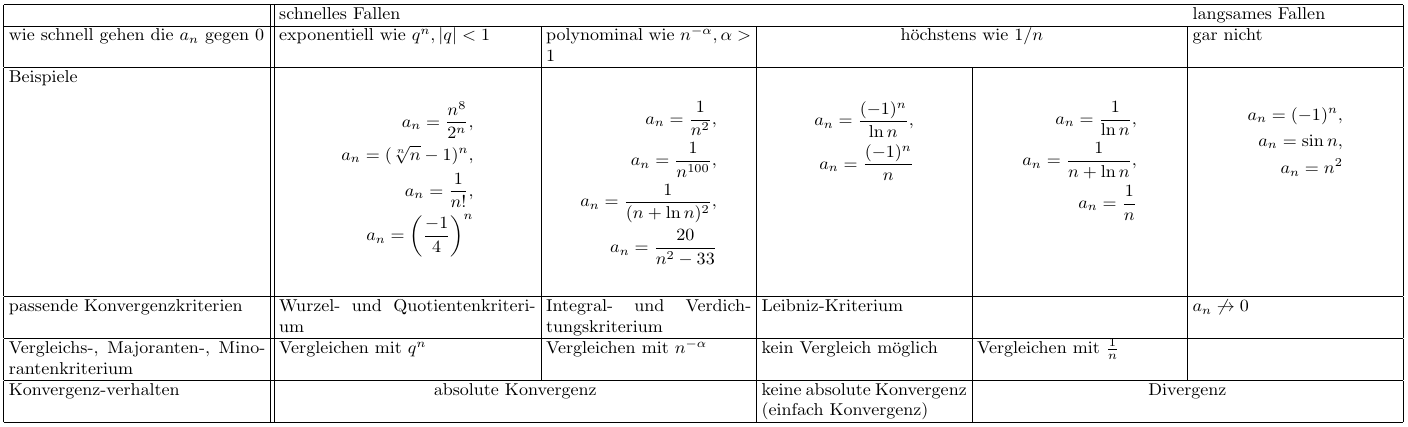
\includegraphics[width=1\textwidth]{images/Reihen_Tables.png}

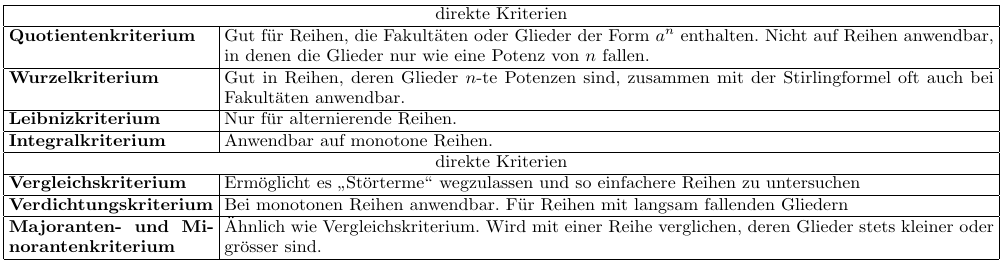
\includegraphics[width=1\textwidth]{images/Reihen_Kriterien.png}
\part{Beispiele}
\setcounter{section}{1}
%\subsection{Beispiel HS19, Residuensatz}

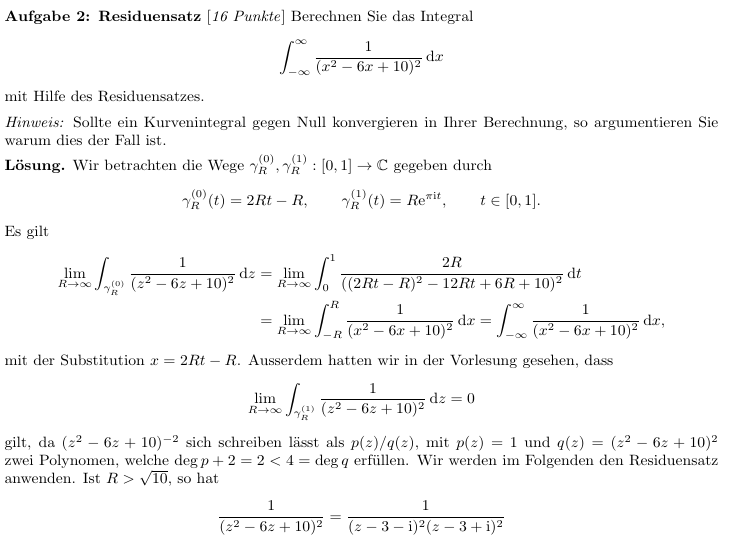
\includegraphics[width=1\textwidth]{images/img_koma/example_1.1_hs19.png}
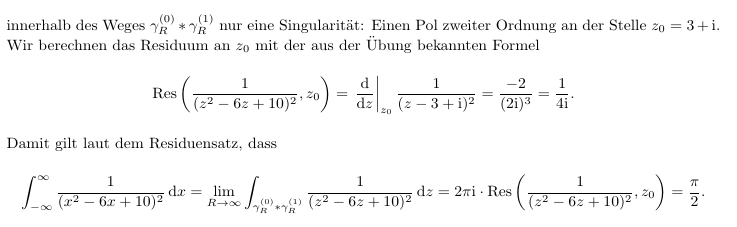
\includegraphics[width=1\textwidth]{images/img_koma/example_1.2_hs19.png}

%\subsection{Beispiel HS19, Laplace-Transform}
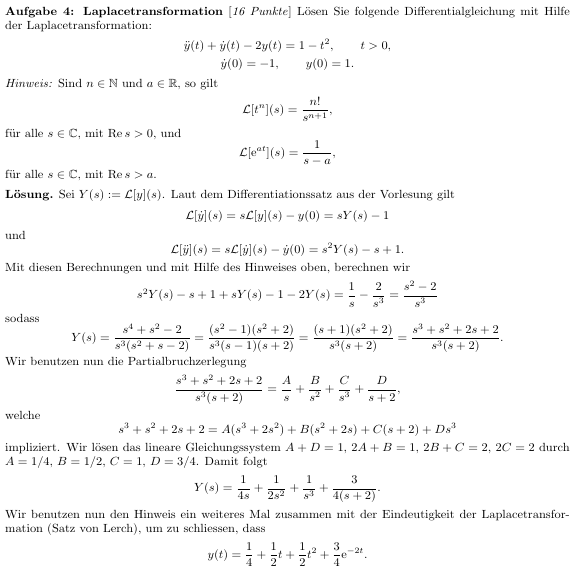
\includegraphics[width=1\textwidth]{images/img_koma/example_1.3_hs19.png}

%\subsection{Beispiel HS19, Fourierreihe}
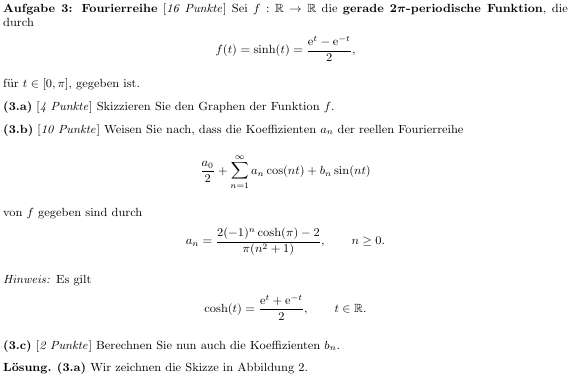
\includegraphics[width=1\textwidth]{images/img_koma/example_1.4.1_hs19.png}
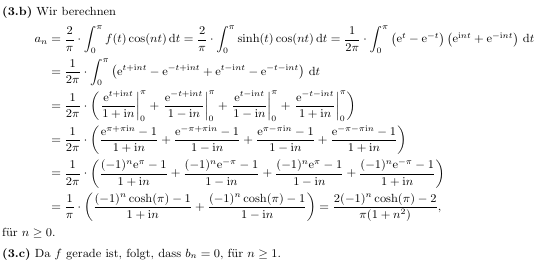
\includegraphics[width=1\textwidth]{images/img_koma/example_1.4.2_hs19.png}
%\footnotesize{Beispiel HS19, Fourierreihe}

%\subsection{Beispiel FS18, Residuensatz}
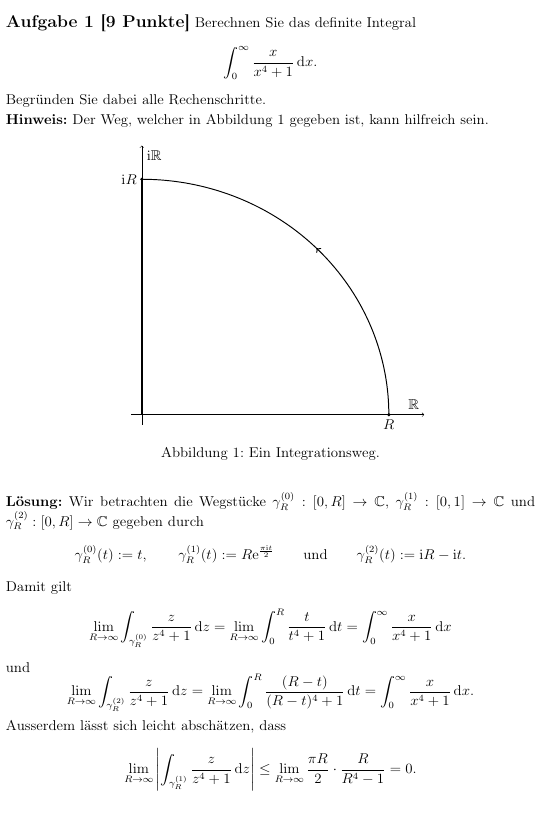
\includegraphics[width=1\textwidth]{images/img_koma/example_1.5.1_fs18.png}
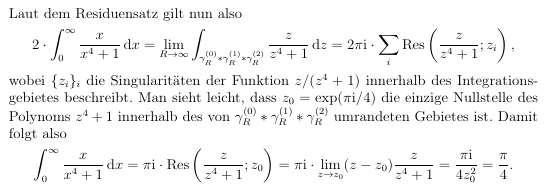
\includegraphics[width=1\textwidth]{images/img_koma/example_1.5.2_fs18.png}


%\subsection{Beispiel FS18, Residuensatz}
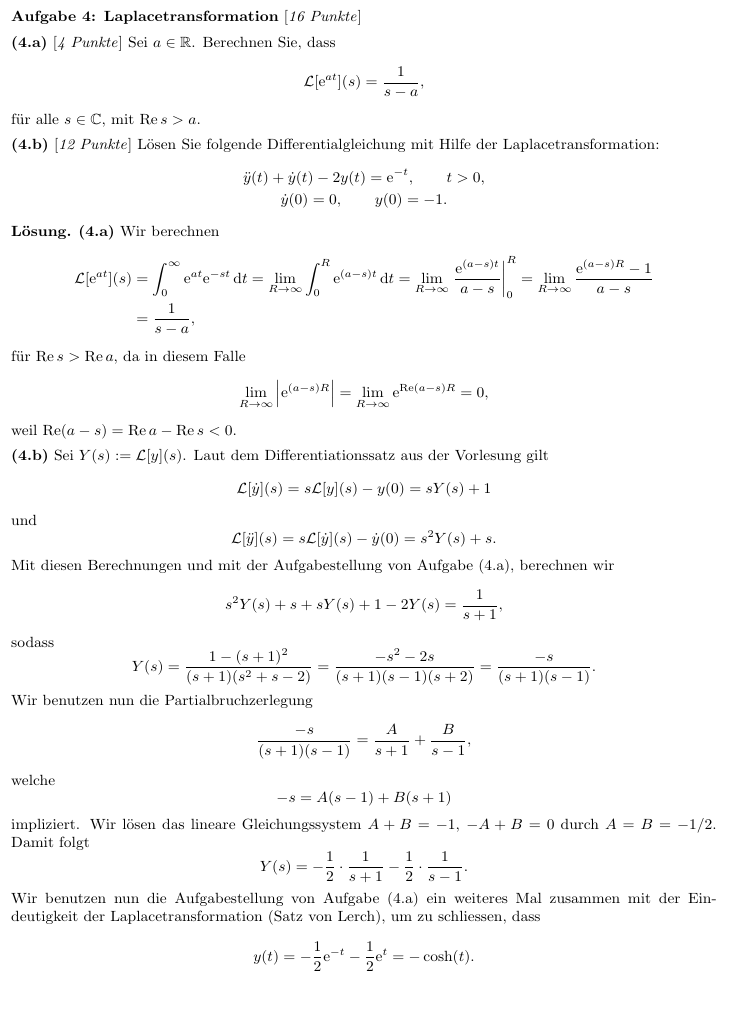
\includegraphics[width=1\textwidth]{images/img_koma/example_1.6_fs19.png}


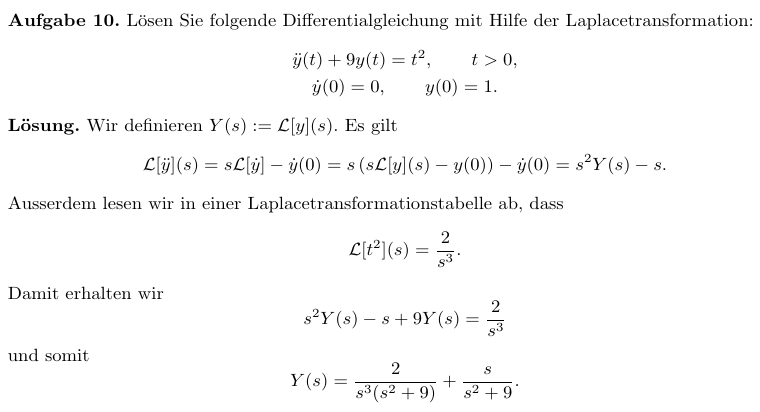
\includegraphics[width=1\textwidth]{images/img_koma/lapl1.png}
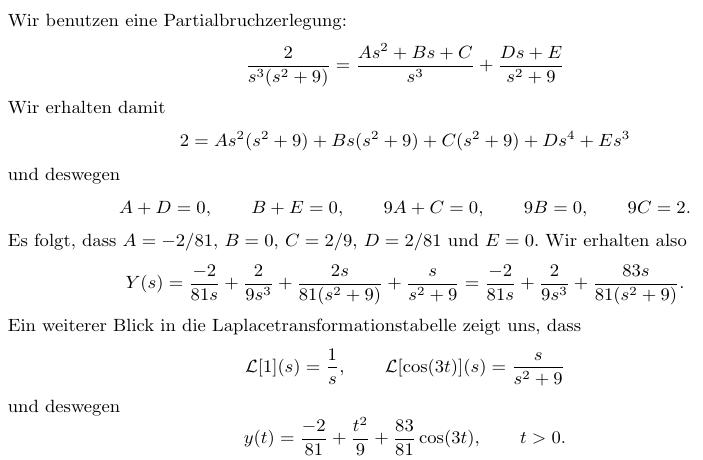
\includegraphics[width=1\textwidth]{images/img_koma/lapl2.png}
Residue\\
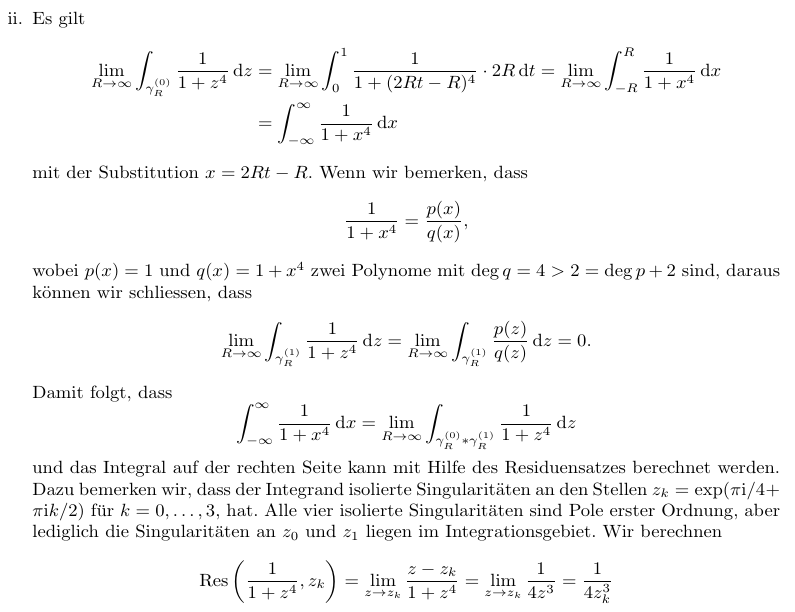
\includegraphics[width=1\textwidth]{images/img_koma/residue1.png}
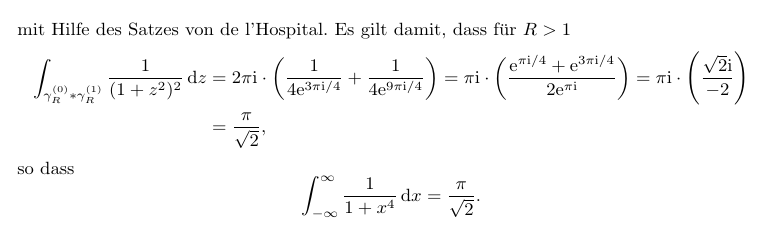
\includegraphics[width=1\textwidth]{images/img_koma/residue2.png}

%\fi


\end{document}


